\documentclass[10pt]{amsart}

\usepackage[margin=1in]{geometry}
\usepackage[T1]{fontenc}
\usepackage{lmodern}
\usepackage{amsmath,amssymb,amsthm,mathtools}
\usepackage{microtype}
\usepackage{url}
\usepackage{enumitem}
\usepackage{alltt}
\usepackage{booktabs}
\usepackage{array}
\usepackage{tikz}
\usepackage[dvipsnames]{xcolor}
\usepackage[colorlinks=true,linkcolor=MidnightBlue,citecolor=OliveGreen,urlcolor=MidnightBlue]{hyperref}
\usepackage[capitalize,nameinlink]{cleveref}

\setlist{leftmargin=*,itemsep=2pt,topsep=4pt}
\emergencystretch=3em
\raggedbottom
\Urlmuskip=0mu plus 1mu

% Theorem environments. The optional note (Lean names and status label) is long, so it is set at the
% start of the body, where it can break across lines, instead of in the unbreakable theorem head.
\theoremstyle{plain}
\newtheorem{thmbase}{Theorem}[section]
\newtheorem{theoremx}[thmbase]{Theorem}
\newtheorem{propositionx}[thmbase]{Proposition}
\newtheorem{corollaryx}[thmbase]{Corollary}
\newtheorem{importedtheoremx}[thmbase]{Imported Theorem}
\newtheorem{conjecturex}[thmbase]{Conjecture}
\newtheorem{questionx}[thmbase]{Question}
\theoremstyle{definition}
\newtheorem{definitionx}[thmbase]{Definition}
\theoremstyle{remark}
\newtheorem{remarkx}[thmbase]{Remark}
\newcommand{\thmnoteinbody}[1]{\if\relax\detokenize{#1}\relax\else{\upshape(#1)}\enspace\fi}
\newcommand{\defthm}[1]{%
  \newenvironment{#1}[1][]{\begin{#1x}\thmnoteinbody{##1}\ignorespaces}{\end{#1x}}}
\defthm{theorem}\defthm{proposition}\defthm{corollary}\defthm{importedtheorem}
\defthm{conjecture}\defthm{question}\defthm{definition}\defthm{remark}
\crefname{theoremx}{Theorem}{Theorems}
\crefname{propositionx}{Proposition}{Propositions}
\crefname{corollaryx}{Corollary}{Corollaries}
\crefname{importedtheoremx}{Imported Theorem}{Imported Theorems}
\crefname{conjecturex}{Conjecture}{Conjectures}
\crefname{questionx}{Question}{Questions}
\crefname{definitionx}{Definition}{Definitions}
\crefname{remarkx}{Remark}{Remarks}
\numberwithin{equation}{section}

\newcommand{\A}{\textup{[A]}}
\newcommand{\Oa}{\textup{[O]}}
\newcommand{\N}{\mathbb{N}}
\newcommand{\Z}{\mathbb{Z}}
\newcommand{\Q}{\mathbb{Q}}
\newcommand{\per}{\operatorname{per}}
\newcommand{\rk}{\operatorname{rank}}
\newcommand{\Bell}{\operatorname{Bell}}
\newcommand{\cost}{\operatorname{cost}}
% Lean names: typewriter, with line breaks allowed after '.' and '_'.
\DeclareUrlCommand\lean{\urlstyle{tt}\def\UrlBreaks{\do\.\do\_}\def\UrlBigBreaks{}}
% Repository names: typewriter, with line breaks allowed after '/' and '-'.
\DeclareUrlCommand\repo{\urlstyle{tt}\def\UrlBreaks{\do\/\do\-\do\.}\def\UrlBigBreaks{}}

\begin{document}

\title[What the ETH refutations do not give]{What the ETH refutations do not give:\\ barriers for the counting engines, with machine-checked lemmas}

\author{Vaibhav Tulsyan}

\date{November 2026}

\subjclass[2020]{68Q17, 68Q25, 68W30, 15A69, 05C31}
\keywords{Exponential Time Hypothesis, counting algorithms, tensor networks, cut rank, permanent, Tutte polynomial, lower bounds for restricted models, Lean~4, formal verification}

\begin{abstract}
In October 2026 OpenAI and Anthropic each claimed a deterministic subexponential algorithm for
counting the solutions of a $k$-CNF; both counting engines sum products of local tables. For SAT
itself, Majdoddin bounds the rate of Anthropic's grid recursions with product terms, and Dias and
Lima bound OpenAI's clause-product scheme. However, Majdoddin notes that no barrier is known for
decompositions whose terms are not products, and neither paper treats the counting problems beyond
SAT. We introduce the \emph{engine barrier problem}: bound from below the shared bits $U$ of every
network of a stated class that computes a given count, and the rate of every recursion of a stated
class. Our approach puts a rank on every cut of a local network, and on one contraction inside both
flattenings of a term. Machine-checked in Lean are: correlated (non-product) decompositions of two
rectangles, of the $3\times2$ grid and of the full $3\times3$ grid level have flattening-rank sums
at least $N^2$, $N^3$ and $N^8$, while $N^9$ is open; the row cut of the permanent has rank $\binom
nk$, which on paper gives $U\ge n\log_2(n/s)$ for row-local networks; algebras in which the
permanent is a functional of a product have dimension at least $\binom n{n/2}$; pieces have saving
$\rho\ge1/2$ (rank form; Anthropic's observation); and exact colouring filters for Hamiltonicity
need $q\ge n-4$ colours. On paper we prove $U\ge(1-o(1))n\log_2n$ for vertex-local networks for the
Tutte polynomial off the integer hyperbolas, and $\rho\ge3/8$ for correlated decompositions of full
grid levels. We cite $45$ Lean theorems, with standard axioms only. Every barrier is about a named
model: in Anthropic's general model no unconditional bound on $U$ exists without separating $\mathrm
P$ from $\mathrm P^{\#\mathrm P}$, and an unconditional cap on oblivious algebraic algorithms would
separate $\mathrm{VP}$ from $\mathrm{VNP}$.
\end{abstract}

\maketitle

% =====================================================================
\section{Introduction}\label{sec:intro}
% =====================================================================

On 26 October 2026 OpenAI~\cite{OpenAI26} and Anthropic~\cite{Anthropic26} (below \Oa{} and \A)
each posted a claimed refutation of the Exponential Time Hypothesis: a deterministic algorithm that
counts the satisfying assignments of a $k$-CNF on $n$ variables in time $2^{O_k(n/\sqrt{\log n})}$ up
to lower-order factors, with a Lean~4 development. Both claims are under review. Both engines are
counting algorithms for sums of products of local tables, and they reach every problem whose
witnesses have $O(n)$ bits and are checked locally. Our earlier work used them, with machine-checked
proofs, for exact counting of Hamiltonian cycles and TSP tours on sparse graphs~\cite{Tul26}, Eulerian
circuits~\cite{TulEuler26}, amplitudes of sparse quantum circuits~\cite{TulQ26},
factoring~\cite{TulFac26}, class numbers~\cite{TulCN26} and the parity of $\pi(x)$~\cite{TulPar26}.

For \#SAT itself, two papers that appeared while this one was in preparation give negative accounts.
Majdoddin~\cite{Maj26} defines a rewrite-and-merge class that contains \A's recursion and proves that
every grid algorithm in it has exponent at least $1/\log_2K$ per edge bit; Dias and Lima~\cite{DL26}
prove that the clause-product form of \Oa's interpolation algorithm costs $2^{\Omega(\sqrt{\mathrm{tw}})}$
at treewidth $\mathrm{tw}$, in a cost model that charges what the preprint pays. The labs' own remarks
are shorter. \A{} writes that its theorem ``does not refute the Orthogonal Vectors hypothesis'' and that
the result ``is purely asymptotic'' (\cref{sec:engines}). \Oa{} notes that a faster algorithm for a
target problem needs ``a reduction in the other direction, from that problem to fixed-width SAT,
that controls the number of variables'', and that ``runtime bounds of the form $2^{o(n)}$ do not
transfer under general polynomial-time reductions''. However, Majdoddin's class requires every term of
a recursion to be a product of one piece per configuration; he calls non-product groupings of terms
the ``open door'' of his class and writes that ``for the full model of Signed Network Sums no barrier
is known''~\cite[\S4.8]{Maj26}. Neither paper treats a counting problem other than (Max-)SAT. We are unaware of a barrier for non-product decompositions, or
of an account of which counting problems beyond SAT the engines cannot be expected to reach, by which
mechanism, and what would have to change. This matters because the engines are new, and the obvious
targets after sparse \#HC (the permanent, dense \#HC and TSP, the chromatic number, the Tutte
polynomial, Subset Sum, exact $\pi(x)$) are exactly the ones they seem to miss.

\subsection{The problem and the running example}
We consider the \emph{engine barrier problem}. For a counting problem $P$ and a stated class of
networks, bound from below the number $U$ of shared bits of every network in the class whose value
is $P$; and for a stated class of recursions, bound from below the rate $e_K$ at which the recursion
evaluates the dense $(K,\lambda)$-clique. The two numbers combine: the engine's own guarantee on a
network is at least $2^{e_K U}$ (\cref{prop:exponent}), and $e_K=\Theta(1/\sqrt{\log K})$ in \A.
So a dense problem is out of reach of the engine's guarantee when $U$ is of order $n\log n$ and $e_K$
is not $o(1/\log K)$. For grid recursions with product terms, $e_K=\Omega(1/\log K)$ is a theorem of
Majdoddin~\cite[Theorem~4.13]{Maj26}; the question we add is what terms that are not products can do.

\begin{figure}[ht]
\centering
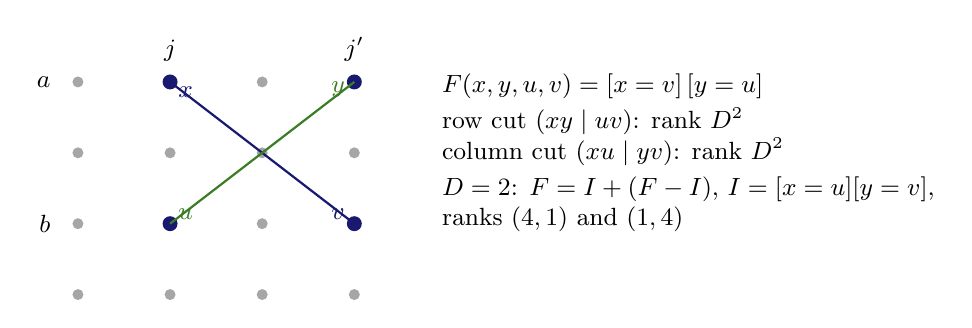
\begin{tikzpicture}[scale=0.9,every node/.style={font=\small}]
  \foreach \i in {0,...,3} \foreach \j in {0,...,3} {
    \fill[black!35] (\j*1.3,-\i*1.0) circle (2.2pt);
  }
  \node[left] at (-0.25,0) {$a$};
  \node[left] at (-0.25,-2.0) {$b$};
  \node[above] at (1.3,0.15) {$j$};
  \node[above] at (3.9,0.15) {$j'$};
  \fill[MidnightBlue] (1.3,0) circle (3pt);
  \fill[MidnightBlue] (3.9,0) circle (3pt);
  \fill[MidnightBlue] (1.3,-2.0) circle (3pt);
  \fill[MidnightBlue] (3.9,-2.0) circle (3pt);
  \draw[MidnightBlue,thick] (1.3,0) -- node[pos=0.18,above left]{$x$} node[pos=0.82,below right]{$v$} (3.9,-2.0);
  \draw[OliveGreen,thick] (3.9,0) -- node[pos=0.18,above right]{$y$} node[pos=0.82,below left]{$u$} (1.3,-2.0);
  \node[right,align=left] at (5.0,-1.0) {$F(x,y,u,v)=[x=v]\,[y=u]$\\[2pt]
    row cut $(xy\mid uv)$: rank $D^2$\\ column cut $(xu\mid yv)$: rank $D^2$\\[2pt]
    $D=2$: $F=I+(F-I)$, $I=[x=u][y=v]$,\\ ranks $(4,1)$ and $(1,4)$};
\end{tikzpicture}
\caption{The running example. One level of \A's recursion evaluates a clique on a $g\times g$ grid of
nodes; each pair of rows $a<b$ and columns $j<j'$ carries a \emph{rectangle}, two crossing equalities
of $\lambda$ bits each. Its tensor $F$ has both flattenings of full rank $D^2$, $D=2^\lambda$. At $D=2$
the split $F=I+(F-I)$ gives two terms, each cheap in one grouping: this is the profile of saving
$\rho=1/2$.}\label{fig:rect}
\end{figure}

\Cref{fig:rect} is our running example. One level of \A's recursion views a clique on $g^2$ nodes as
a $g\times g$ grid. Each pair of rows and pair of columns spans a rectangle with corner legs
$x,y,u,v\in[D]$ and tensor $F=[x=v][y=u]$. Evaluated row by row, a term costs the rank of its row
flattening $(xy\mid uv)$; evaluated column by column, the rank of its column flattening
$(xu\mid yv)$. For $F$ both are permutation matrices of rank $D^2$. The recursion therefore splits $F$
into \emph{pieces}, terms that are cheap in one of the two groupings, and the saving $\rho$ per level
decides its rate. At $D=2$ the split $F=I+(F-I)$ has rank profiles $(4,1)$ and $(1,4)$: each piece
pays $2$ bits in one grouping and none in the other, half of the $4$ bits of $F$. We come back to this
example in \cref{sec:engines} (what a shared bit buys) and in \cref{sec:rate}: on two rectangles and on
the $3\times2$ grid no decomposition, correlated or not, does better asymptotically, and on the
$3\times3$ level the question is open.

\subsection{The naive route and the principle}
At first one might try to prove that the dense permanent needs $2^{\Omega(n)}$ steps in the engine,
for example by bounding $U$ from below for every network whose value is $\per(A)$. However, in \A's
Definition~2 the node tables are arbitrary polynomial-time functions of the whole input; Ryser's
formula is then a one-node network with $U=0$, and a network with $U=0$ and one setting exists if and
only if $\per\in\mathrm{FP}$ (\cref{prop:general}). Instead, we rely on a different principle:
\emph{every known network is local, and locality lets a cut carry a rank.} If the nodes on one side
of a cut read one part of the input and the nodes on the other side read the rest, then the value,
as a matrix indexed by the two parts, has rank at most $2^w$, where $w$ is the number of shared bits
across the cut. The same rank argument bounds the cost of a term of a recursion through its two
flattenings, as in \cref{fig:rect}.

In Anthropic's general network model a node table may be any polynomial-time function of the whole
input, so no unconditional lower bound on shared bits is possible without separating $\mathrm P$
from $\mathrm P^{\#\mathrm P}$ (\cref{prop:general}); every theorem of this paper is about a named
class of local networks or recursions.

\subsection{What we do}
In this paper we define the models (row-local and vertex-local networks, pieces, grouping
recursions, correlated decompositions, \Oa's $M_0$-template, tree verifiers), prove rank lower bounds
in each, and assemble them into a map of nine problems. The key observation is that the two numbers
$U$ and $e_K$ are each controlled by one rank: $U$ by the rank of the value across a cut of the
input, and $e_K$ by the rank of a contraction that is a submatrix of both flattenings of a term at
once. Many ingredients are classical: Nisan's rank characterisation of noncommutative branching
programs~\cite{Nisan91}, Lindstr\"om's factorisation of meet matrices~\cite{Lindstrom69}, and rank
subadditivity. The product-term caps of \cref{sec:pieces,sec:groupings} are parallel to, and weaker
than, Majdoddin's~\cite{Maj26}. What is new is the correlated decompositions of
\cref{sec:correlated}, the walls for the problems beyond SAT (\cref{sec:wall,sec:encodings,sec:map}),
and a Lean development that checks every rank statement we cite.

\subsection{Contributions}
Our contributions are:
\begin{itemize}
\item We introduce the engine barrier problem and its two numbers, and define the network and
recursion models in which we bound them (\cref{sec:engines}).
\item We prove that dense counting costs $\Omega(n\log n)$ shared bits in the local networks we can
analyse: $U\ge n\log_2(n/s)$ for row-local networks for the permanent (rank and counting steps in
Lean), $\binom n{n/2}$ for algebras (Lean), and, on paper, $(1-o(1))\,n\log_2 n$ for vertex-local
networks for the Tutte polynomial off the integer hyperbolas (\cref{sec:wall}).
\item We prove, to our knowledge, the first barriers for correlated (non-product) decompositions,
the region that Majdoddin's class leaves open: rank sums at least $N^2$, $N^3$ and $N^8$ on two
rectangles, the $3\times2$ grid and the $3\times3$ level (Lean, rank form), $\rho\ge3/8$ on full levels
(on paper), and a proof that flattening certificates stop at $8$ on the $3\times3$ level
(\cref{sec:correlated}).
\item We machine-check the rank form of $\rho\ge1/2$ for pieces (\A's Appendix~H observation,
generalised in~\cite{Maj26}), and prove on paper $\rho\ge1/\sqrt2-o(1)$ for graded two-order pieces
and $\alpha'\le1$ for every family of groupings of the grid rectangles
(\cref{sec:pieces,sec:graded,sec:groupings}); and we prove that \Oa's $M_0$-template is tight at
$R\approx\sqrt Q$ (\cref{sec:openai}).
\item We prove floors for three of our own linear encodings of Hamiltonicity: $q\ge n-4$ colours,
$k^*(H_t)\ge(\log_2t-10)/20$ turn bits, and a support threshold $t_p\le\log_2\#S$ below which
every residue query vanishes (Lean, \cref{sec:encodings}).
\item We map nine problems out of reach (\cref{tab:map}, \cref{sec:map}), state what would have to
change and why proving that it will not is itself out of reach (\cref{sec:change}), and describe the
Lean development: $45$ cited theorems in $16$ modules (\cref{sec:lean}).
\end{itemize}

\subsection{Status of each claim}\label{sec:status}
We separate four kinds of claim, and every theorem environment carries its label.
\emph{Machine-checked in Lean} (\textsc{Theorem}, ``machine-checked''): the $45$ statements named in
\cref{sec:lean}, with the axioms \texttt{propext}, \texttt{Classical.choice} and \texttt{Quot.sound}
only. Two of them have hypotheses that stand for steps proved on paper
(\cref{thm:modelR,thm:tree}), and the bracket says so; the hypothesis of \cref{thm:colourpoly} is
discharged in Lean by \cref{thm:colour}. The Lean statements about
correlated decompositions bound ranks of flattenings; the step ``a network of cost $c$ has
flattening rank at most $2^c$'' is on paper.
\emph{Proved on paper only} (\textsc{Proposition}, ``on paper'', with the research note and its own
number): the engine exponent (\cref{prop:exponent}), the general-model statement
(\cref{prop:general}), Model~V and the Tutte barrier (\cref{prop:modelV,prop:tutte}), the entropy
bounds for $\#$SAT encodings (\cref{prop:entropy}), the graded two-order bound and the grouping caps
(\cref{prop:graded,prop:twogroup,prop:covering,prop:multigroup}), the full-level bound
$\rho\ge3/8$ and its limit (\cref{prop:fulllevel,prop:limit}), the template bounds
(\cref{prop:template}), the black-box and adversary statements, the accounting for Subset Sum and
products (\cref{prop:subsetsum,prop:circuit}), and the meta-barrier and conditional cap
(\cref{prop:meta,prop:hlog}).
\emph{Assumed}: the statements of \A{} and \Oa{} that we quote as Imported Theorems, pinned to
commits and sections. They enter only as the object our barriers are about; no barrier of this paper
depends on their correctness.
\emph{Checked numerically} (\textsc{Remark}, ``checked numerically''): exact rank tables, the
$\lambda=1$ searches and the integer programs of \cref{sec:correlated}. They never support an
asymptotic claim. No theorem in this paper is about all algorithms.

\subsection*{Outline}
\Cref{sec:engines} recalls the engines and defines the models. \Cref{sec:wall} proves the
$n\log n$ wall for shared bits, \cref{sec:rate} the caps on the rate and \cref{sec:openai} the
tightness of \Oa's template. \Cref{sec:encodings} treats our own encodings, \cref{sec:map} the nine
problems and \cref{sec:change} what would have to change. \Cref{sec:lean} describes the Lean
development, and \cref{sec:related,sec:limitations,sec:conclusion} cover related work, limitations
and conclusions.

% =====================================================================
\section{The engines and their two numbers}\label{sec:engines}
% =====================================================================

In this section we recall the statements of \A{} and \Oa{} that our barriers are about, define the
network models, and prove on paper that the engine's guarantee on a network is at least
$2^{e_KU}$. We use \A's development at commit \texttt{16a5ce4} (\texttt{anthropics/formal-math},
folder \texttt{eth}) and \Oa's at commit \texttt{7ef5c0c} (\texttt{openai/math}, preprint revised
25~October 2026). Logarithms are to base $2$.

\paragraph{The labs' own limits.} \A, Introduction: ``Theorem~1 does not refute the Orthogonal Vectors
hypothesis, which SETH implies and on which many lower bounds in fine-grained complexity rest'', and
``Our result is purely asymptotic''. \Oa, \S1.1.3 (``Implications for fine-grained complexity''):
lower bounds that ``follow from the hypothesis that unrestricted CNF-SAT admits no
$2^{(1-\delta)n}\mathrm{poly}(n,m)$-time algorithm'' survive, since its theorem ``gives a
running-time guarantee for each fixed clause width $k$, while this hypothesis allows the width to
grow with $n$''; and ``to obtain a faster algorithm for a target problem from our SAT algorithm, we
need a reduction in the other direction''. In the remark before its corollary on graph counting,
\Oa{} adds that ``runtime bounds of the form $2^{o(n)}$ do not transfer under general polynomial-time
reductions''. For SAT itself Majdoddin~\cite{Maj26} and Dias and Lima~\cite{DL26} give negative
accounts; this paper gives one for the problems beyond SAT and for non-product decompositions.

\subsection{Networks and shared bits}
\begin{definition}[Networks; \A, Definition~2]\label{def:network}
A \emph{network} on $[g]$ has, for every node $a$, a set $S_a$ of settings of at most $P$ bits and a
weight table $W_a$, and for every pair $a\ne b$ an interaction $\Psi_{a,b}$ that factors through
$c_{a,b}$ shared bits: $\Psi_{a,b}(z,z')=\sum_{\theta\in\{0,1\}^{c_{a,b}}}f_{a,b}(z,\theta)f_{b,a}(z',\theta)$.
Its value is $\sum_{z}\prod_aW_a(z_a)\prod_{a<b}\Psi_{a,b}(z_a,z_b)$, and its total is
$U=\sum_a\sum_{b\ne a}c_{a,b}$, so every shared bit is counted at both ends. The \emph{skeleton} is
$(g,(c_{a,b}))$. A \emph{network family} for a counting problem is a map from inputs to networks
whose value is the count.
\end{definition}

In \A{} the tables are given by polynomial-time procedures that see the whole input. The known
networks are local: in \A's $3$-SAT network a node reads the clauses of one block, and in our
Hamiltonian-cycle network a node reads the edges at one vertex cluster. Two locality classes carry
our theorems.

\begin{definition}[Model~R$(s)$ and Model~V$(s)$; \repo{barrier.md} Definitions~5.1, 5.2]\label{def:models}
Let the input be a matrix $A\in\{0,1\}^{n\times n}$ (or a graph on $[n]$). In \emph{Model~R$(s)$} the
rows are partitioned into clusters of size at most $s$, every node is assigned to one cluster or is a
routing node that reads nothing, the skeleton does not depend on $A$, and the data of a node depend
on $A$ only through the rows of its cluster. In \emph{Model~V$(s)$} the $2n$ rows and columns (or the
$n$ vertices) are partitioned into clusters of size at most $s$, and the data of a node depend only on
the entries in the rows and columns of its cluster (the edges with an end in it); otherwise as before.
\end{definition}

\subsection{The engine of \A}
\begin{importedtheorem}[\A, Lemma~8(i), Theorem~A and Theorem~B; imported, not used as an assumption]\label{imp:engine}
Let $K\ge2$, $g=3K^8$. A network on $[g]$ with parameters $P,B,\tau$ and total $U$ is evaluated within
$(K^g+T\cdot2^{2gP/K}\tau)(g(P+B))^{C_1}$ operations, where $T$ bounds the cost of a $(K,L)$-clique
with $L=\lceil(U+gP/K)/K^2\rceil$ (Lemma~8(i), Lean \texttt{ExplicitCost.groupingExplicit}). If pieces
with parameters $(\rho,c)$ exist, one algorithm evaluates the $(K_\ell,\lambda)$-clique within
$2^{e_\ell K_\ell^2\lambda}(K_\ell(\lambda+B))^{C_0K_\ell^2}$ operations, where
$\log K_\ell=(3x_0+6)2^\ell-6\ell-2x_0-6$ and $\tfrac12\rho^\ell\le e_\ell\le0.85\rho^\ell$, $x_0\ge18$
(Theorem~A, Lean \texttt{ExplicitCost.recursionSolves}). Pieces with $\rho=1/\sqrt2$ exist
(Theorem~B, Lean \texttt{PiecesCounted.halfPieces}).
\end{importedtheorem}

The $(K,\lambda)$-clique $C(K,\lambda)$ is the network on $K$ nodes in which every pair shares one
$\lambda$-bit label through $\Psi_{w,w'}=[z_w(w')=z_{w'}(w)]$, with arbitrary tables. Its cost is
written $2^{e_KK^2\lambda}$; brute force has $e_K=(K-1)/(2K)$. One level of Theorem~A maps a
$(g^2,\lambda)$-clique, viewed as the $g\times g$ grid of \cref{fig:rect}, to networks on $g$ nodes
grouped by rows or by columns. The straight edges inside a row or column cost $O(N/g)$ of the
$N=g^4\lambda$ shared bits; the rest sits on the $\binom g2^2$ rectangles. A \emph{family of pieces}
writes $d\cdot F=\sum_{i\in I}A_i$ with $|I|\le(2\lambda)^c$ and certified costs
$c^{\mathrm{row}}_i,c^{\mathrm{col}}_i$ with $c^{\mathrm{row}}_i+c^{\mathrm{col}}_i\le4\rho\lambda+c\log(2\lambda)$
(\A, Definition~7). Every term $\iota\in I^R$ of the expansion of $\prod_qF_q$ is a row network and a
column network, and the level pays the cheaper one, which saves the factor $\rho$. Since
$K_{\ell+1}\ge K_\ell^2$ while $e$ drops by $\rho$, the rate is $e_K\asymp(\log K)^{-\alpha'}$ with
$\alpha'=\log_2(1/\rho)$; $\rho=1/\sqrt2$ gives $\alpha'=1/2$.

\paragraph{What a shared bit buys.} In \cref{fig:rect} a rectangle carries $4\lambda$ shared bits at both
ends. A piece with $(c^{\mathrm{row}},c^{\mathrm{col}})=(2\lambda,0)$ costs nothing in the column grouping,
and at $D=2$ the split $F=I+(F-I)$ realises the profile $\{(2,0),(0,2)\}$, i.e.\ $\rho=1/2$. For
larger $D$ the same split does not keep this profile ($F-I$ has row rank $D(D-1)/2$), and \A's
Theorem~B pays $1/\sqrt2$ instead. The question of \cref{sec:rate} is whether any decomposition
beats $1/2$; the question of \cref{sec:wall} is how many rectangles, that is how many shared bits, a
dense problem forces.

\subsection{The engine of \Oa}
\Oa's Theorem~1.1 counts the solutions of a $k$-CNF with $m$ clauses in time
$(n+m)^{O_k(1)}2^{O_k(n\log\log n/\sqrt{\log n})}$ and polynomial space. Its Engine~I needs a
\emph{layout} (\Oa, Definition \texttt{def:layout}; Lean \texttt{LayoutSpec.Layout}): partitions of the
variables at $Q$ interpolation points, schedules for the factors, measurement matrices of small
$\ell_1$ height, and for every occurrence a row polynomial $P_{f,v}(T)$ of degree at most $R$ with
$P_{f,v}(0)=\delta_v$ that annihilates the measurement kernels of the other groups. The cost exponent
is about $n[(R/Q)\log(2Q/R)+\tau\log(2D+1)+2/r]$. \Oa's construction (its \S4) is a template: a
matrix $M_0$ acting on labels in $[r]^Q$, with support condition~(T2), $M_0[u,w]\ne0\Rightarrow
d_H(d_u,a_w)\le R-1$. \Cref{sec:openai} bounds every instance of this template.

\subsection{The engine exponent}
\begin{proposition}[on paper; \repo{barrier.md} Lemmas~2.0, 2.1, 2.2]\label{prop:exponent}
Let $N$ be a network with total $U\ge1$ to which Lemma~8 is applied with any admissible $K$ and the
clique algorithm of Theorems~A(b) and B. Then the guaranteed running time is at least $2^{E(N)}$ with
\[
  E(N)\ \ge\ e_KU+2gP/K\ \ge\ \frac{U}{2\sqrt{\log U+2x_0}}.
\]
So the guarantee is below $2^n$ only if $U<(2+o(1))\,n\sqrt{\log n}$, and with pieces of saving
$\rho\ge1/2$ it is at least $2^{U/(2(\log U+2x_0))}$. Any algorithm for the $(K,\lambda)$-clique that
reads its tables has $e_K\ge(K-1)/K^2-o(1)$, which alone gives only $E(N)\ge\sqrt{2U}(1-O(1/K))$.
\end{proposition}

\noindent The proof reads $e_K\ge1/(2\sqrt{\log K+2x_0})$ off Theorem~A(a), notes $K^2L\ge U$ and
$2gP/K\ge2K$, and splits on whether $2K$ exceeds the bound. The query bound $(K-1)/K^2$ is Majdoddin's
input floor~\cite[Proposition~2.4(a)]{Maj26} in our normalisation (his exponent is per edge bit, of
which the clique has $\binom K2\lambda$). The last sentence is the reason
\cref{sec:rate} matters: with a hypothetical optimal clique solver, no lower bound on $U$ of order
$n\log n$ would bar anything. This proposition is about \A's guarantee as a function of $U$, for all
inputs; it is one of the three places (with \cref{sec:openai} and \cref{cor:Bprime}) where a
statement concerns the engines as published rather than a class of networks.

% =====================================================================
\section{Dense counting costs \texorpdfstring{$n\log n$}{n log n} bits in every local network we can analyse}\label{sec:wall}
% =====================================================================

In this section we prove the lower bounds on $U$. We first state the cut lemma in rank form
(\cref{sec:cut}), then compute the rank of the permanent across a row cut (\cref{sec:rowcut}), and
sum the cuts in Model~R (\cref{sec:modelR}) and Model~V (\cref{sec:modelV}). \Cref{sec:algebra}
treats algebras and characteristic~$p$, \cref{sec:tutte} the Tutte plane, and \cref{sec:general} says
why no such bound exists in the general model.

\subsection{The cut lemma}\label{sec:cut}
Let $N$ be a network and $(L,R)$ a partition of its nodes, with $w(L,R)=\sum_{a\in L,b\in R}c_{a,b}$
crossing bits. Replacing every crossing interaction by its factorisation and exchanging the sums gives
$\mathrm{value}(N)=\sum_{\theta\in\{0,1\}^{w}}F_L(\theta)F_R(\theta)$, where $F_L$ depends only on the
data of the nodes in $L$ (\repo{barrier.md} Lemma~3.1, on paper). So if the nodes in $L$ read only a
part $X$ of the input and those in $R$ only the rest $Y$, the matrix $[\mathrm{value}(N(X,Y))]_{X,Y}$
factors through $2^w$ terms. The rank form is machine-checked.

\begin{theorem}[\lean{EthFollowup.Barriers.Rank.rank_le_card_of_eq_sum_mul}, \lean{EthFollowup.Barriers.Rank.rank_le_two_pow_of_eq_sum_mul}, \lean{EthFollowup.Barriers.Rank.rank_eq_card_of_linearIndependent}; machine-checked]\label{thm:cut}
Let $K$ be a field and $X,Y,\Theta$ types with $Y$ and $\Theta$ finite.\footnote{Module
\repo{lean/EthFollowup/Barriers/RankBounds.lean}.} If $M[x,y]=\sum_{\theta\in\Theta}F(x,\theta)G(\theta,y)$
for all $x,y$, then $\rk M\le|\Theta|$; for $\Theta=\{0,1\}^w$ this is $\rk M\le2^w$. If moreover
$M[x,y]=\sum_{t\in T}u_t(x)v_t(y)$ over a finite $T$ with both families $(u_t)$, $(v_t)$ linearly
independent ($X,Y$ finite), then $\rk M=|T|$.
\end{theorem}
\begin{proof}
Write $M=\mathcal F\mathcal G$ with $\mathcal F=[F(x,\theta)]$ and $\mathcal G=[G(\theta,y)]$; the rank of a
product is at most its inner dimension $|\Theta|$. For the second statement, $M=UV^{\mathsf T}$ with $U$
and $V$ of full column rank $|T|$.
\end{proof}

\subsection{The permanent's row cut}\label{sec:rowcut}
\begin{theorem}[\lean{EthFollowup.Barriers.RowCut.rowCut_rank}, \lean{EthFollowup.Barriers.RowCut.rowCut_rank_oneHot}, \lean{EthFollowup.Barriers.RowCut.permanent_joinMat}; machine-checked]\label{thm:rowcut}
Let $K$ be a field, $\iota$ a finite type with $n$ elements and $I\subseteq\iota$ with
$|I|=k$.\footnote{Module \repo{lean/EthFollowup/Barriers/RowCut.lean}.} Let $M_I$ be the matrix whose rows are
indexed by the $0/1$ rows $X:I\to\iota\to\{0,1\}$, whose columns are indexed by
$Y:I^c\to\iota\to\{0,1\}$, and whose entry is $\per(X;Y)$, the permanent of the matrix with rows $I$
read from $X$ and the other rows from $Y$. Then $\rk M_I=\binom nk$, and the same holds for the
submatrix on one-$1$-per-row matrices. The proof is the Laplace expansion
$\per(X;Y)=\sum_{|S|=k}U_S(X)V_S(Y)$ along the rows $I$.
\end{theorem}
\begin{proof}
A permutation of $\iota$ maps $I$ onto some $S$ with $|S|=k$, which gives the Laplace expansion. Evaluated
at the one-$1$-per-row matrix $X$ that matches $I$ onto $S_0$, $U_S(X)=[S=S_0]$, so the $U_S$ are
linearly independent, and likewise the $V_S$; \cref{thm:cut} gives rank exactly $\binom nk$, already on
the one-$1$-per-row family.
\end{proof}

\noindent An aside, not part of the statement above: on one-$1$-per-row matrices the permanent
$\per(X;Y)$ is the indicator that $(X;Y)$ is a permutation matrix, so on that family the rank statement
is about this indicator.

\subsection{Model~R: \texorpdfstring{$U\ge n\log(n/s)$}{U >= n log(n/s)}}\label{sec:modelR}
For a cluster $j$ of Model~R$(s)$, cut the nodes into those of cluster $j$ and the rest. The left side
reads the rows $V_j$ and the right side the other rows, so \cref{thm:cut,thm:rowcut} give
$\binom n{|V_j|}\le2^{w_j}$ with $w_j$ the bits crossing that cut; this step, from a network to a
factorisation, is on paper. Each ordered pair of nodes is counted in at most one $w_j$, which is
machine-checked, and the rest is arithmetic.

\begin{theorem}[\lean{EthFollowup.Barriers.Rank.modelR_bound_nlogn}, \lean{EthFollowup.Barriers.Rank.modelR_bound}, \lean{EthFollowup.Barriers.Rank.sum_crossing_le_total}; machine-checked with hypotheses \texttt{hrank} and \texttt{hU} on paper]\label{thm:modelR}
Let $J$ be a finite set of clusters, $n,s,U\in\N$, and $k,w:J\to\N$ with $1\le k_j\le s$ and
$\sum_jk_j=n$. Assume \texttt{hrank}: $\binom n{k_j}\le2^{w_j}$ for every $j$ (the cut lemma with the
row cut, on paper for a given network), and \texttt{hU}: $\sum_jw_j\le U$. Then
\[
  n\log_2(n/s)\ \le\ \sum_{j}\log_2\binom n{k_j}\ \le\ U.
\]
The second inequality needs only \texttt{hrank} and \texttt{hU} (\lean{modelR_bound}). For
\texttt{hU}: for every assignment $\mathrm{cl}$ of nodes to clusters or routing and every $c$,
$\sum_{j}\sum_{a,b}[\mathrm{cl}(a)=j\ne\mathrm{cl}(b)]\,c_{a,b}\le\sum_{a\ne b}c_{a,b}$
(\lean{sum_crossing_le_total}), so \texttt{hU} holds with $w_j$ the crossing bits of cluster $j$.
\end{theorem}

\noindent Assembled on paper (\repo{barrier.md} Theorem~6.1): every network family for $\per$ in
Model~R$(s)$ has $U\ge n\log_2(n/s)$, already if the value is correct only on one-$1$-per-row
matrices; with \cref{prop:exponent}, for $s\le n^{1-\varepsilon}$ the engine's guarantee on any such
network is $2^{\omega(n)}$ (\repo{barrier.md} Corollary~6.3). This is the analogue of Nisan's bound
for noncommutative branching programs~\cite{Nisan91}, with row-locality in place of the variable order.

\subsection{Vertex-local networks: trees and the single-cut limit}\label{sec:modelV}
In Model~V a node also reads the columns of its cluster, and the row-cut argument breaks: each side
sees part of the other's input. A vertex cut with $k$ rows and $k$ columns on the small side has
rank exactly $\binom{2k}k$ for a suitable fixing of the shared entries, by the Vandermonde identity.

\begin{theorem}[\lean{EthFollowup.Barriers.Rank.treeSkeleton_bound}, \lean{EthFollowup.Barriers.Rank.sum_choose_mul_choose}; machine-checked with hypothesis \texttt{hrank} on paper]\label{thm:tree}
Let $E$ be a finite set of tree edges and $U\in\N$, $c,k,k':E\to\N$, with $U=2\sum_ec_e$. Assume
\texttt{hrank}: $\binom{k_e+k'_e}{k_e}\le2^{c_e}$ for every edge $e$ (the cut lemma with the vertex-cut
rank, on paper). Then $2\sum_e\log_2\binom{k_e+k'_e}{k_e}\le U$. Also
$\sum_{i=0}^{k}\binom ki\binom{k'}i=\binom{k+k'}k$ for all $k,k'$.
\end{theorem}

\begin{proposition}[on paper; \repo{barrier.md} Theorem~6.2 and Proposition~3.5, \repo{vertex-local-bound.md} Theorems~2.1, 3.1, Corollary~3.2, Propositions~4.1, 4.2]\label{prop:modelV}
Every network family for $\per$ in Model~V$(s)$ has $U\ge2n-o(n)$ for $s\le n^{1/3}$. No single cut gives
more: for a vertex cut with $k$ rows and $k$ columns on the small side, every fixing of the other
entries gives rank at most $\binom{2k}k<4^k$. If the skeleton is a tree of maximum degree $\Delta$ with
the clusters $\{i,i'\}$, then $U\ge(4/\log_2(\Delta-1))\,n\log_2n-O(n\log\log n)$. On the clusters
$\{i,i'\}$, no star skeleton with one shared bit per leaf computes $\per$ for $n\ge3$. The function
$[A\text{ is a permutation matrix}]$ has a Model~V$(1)$ network with $U=0$ but needs
$U\ge n\log(n/s)$ in Model~R$(s)$, so the one-$1$-per-row family gives no bound in Model~V.
\end{proposition}

\noindent The star statement uses Cayley's hyperdeterminant and is checked numerically for $n=3,4$;
the Catalan cut rank of the family $\{I+P_\sigma\}$ is checked for $b\le5$.
\begin{conjecture}[Model~V; \repo{barrier.md} Conjecture~6.5]\label{conj:modelV}
Every network family for $\per$ in Model~V$(s)$ has $U\ge(1-o(1))\,n\log_2(n/s)$. Proved: $2n-o(n)$ for
$s\le n^{1/3}$, and $(4/\log_2(\Delta-1)-o(1))\,n\log_2n$ for trees of bounded degree; the star with two
bits per leaf is the first skeleton on which every cut passes.
\end{conjecture}

\subsection{Substitution algebras and characteristic \texorpdfstring{$p$}{p}}\label{sec:algebra}
A different way to evaluate $\per$ is to substitute ring elements for the entries and read a
coefficient, as Clifford, group-algebra and Kronecker tricks do.

\begin{theorem}[\lean{EthFollowup.Barriers.AlgebraRank.algebra_rank_half}, \lean{EthFollowup.Barriers.AlgebraRank.algebra_rank_sum}; machine-checked]\label{thm:algebra}
Let $K$ be a field and $R$ a finite-dimensional $K$-algebra, not necessarily
commutative.\footnote{Module \repo{lean/EthFollowup/Barriers/AlgebraRank.lean}.} Let
$\varphi:R\to K$ be $K$-linear and $r_{ij}\in R$ ($i,j<n$) with
$\varphi(r_{0f(0)}r_{1f(1)}\cdots r_{n-1,f(n-1)})=[f\text{ bijective}]$ for every $f:[n]\to[n]$. Then
$\binom n{\lfloor n/2\rfloor}\le\dim_KR$. For finitely many such algebras $A_t$ with
$\sum_t\varphi_t(r^{(t)}_{0f(0)}\cdots r^{(t)}_{n-1,f(n-1)})=[f\text{ bijective}]$,
$\binom n{\lfloor n/2\rfloor}\le\sum_t\dim_KA_t$.
\end{theorem}
\begin{proof}
For $|S|=n/2$ let $u_S$ be the product of the first $n/2$ factors along a fixed bijection onto $S$, and
$v_S$ the product of the last $n/2$ along a bijection onto the complement. Then
$\varphi(u_Sv_{S'})=[S=S']$, so the $\binom n{n/2}$ elements $u_S$ are linearly independent in $R$. For
several algebras apply this to the product algebra with the functional $\sum_t\varphi_t$.
\end{proof}

\begin{theorem}[\lean{EthFollowup.Barriers.PermModP.permanent_eq_zero_of_low_rank}; machine-checked]\label{thm:modp}
Let $R$ be a commutative ring of characteristic $p$, $p$ prime, and $\iota,\kappa$ finite
types.\footnote{Module \repo{lean/EthFollowup/Barriers/PermModP.lean}.} If $A=UV^{\mathsf T}$ with
$U,V\in R^{\iota\times\kappa}$ and $|\kappa|(p-1)<|\iota|$, then $\per A=0$.
\end{theorem}
\begin{proof}
Expanding $A=UV^{\mathsf T}$ column by column gives $\per A=\sum_{\ell:\iota\to\kappa}\bigl(\prod_iV_{i\ell(i)}\bigr)\per U_\ell$,
where column $i$ of $U_\ell$ is column $\ell(i)$ of $U$. If $|\kappa|(p-1)<|\iota|$, some value of $\ell$ is
taken at least $p$ times, so $U_\ell$ has $p$ equal columns; a $p$-cycle permuting them acts freely on the
terms of $\per U_\ell$ and leaves each orbit sum $p$ times one term, which is $0$ in characteristic $p$.
\end{proof}

\noindent So every saving that characteristic $p$ gives through low rank dies once $p$ is of order $n$,
and the Chinese remainder theorem needs primes up to about $0.9\,n\ln n$.

\begin{proposition}[on paper; \repo{wild-ideas.md} F1, \repo{perm-mod-p.md} Lemma~B4]\label{prop:entropy}
If $\per(A)=\sum_{t\le T}w_t\,\#\mathrm{SAT}(F_t)$ for all $0/1$ matrices $A$, with integers
$|w_t|\le2^W$, then some $F_t$ has at least $\log_2n!-W-\log_2T=n\log_2n-1.45n-W-\log_2T$ variables.
The same holds modulo any $M$ with $\log_2M\ge\log_2n!+2$.
\end{proposition}

\noindent So plain $\#$SAT encodings of $\per$ have $n\log n-O(n)$ variables, where the Lean
$\#k$-SAT bounds of both labs cost $2^{\Theta(n\sqrt{\log n}\log\log n)}$ or more.

\subsection{The Tutte plane off the hyperbolas}\label{sec:tutte}
Write $q=(x-1)(y-1)$, $H_q=\{(x,y):(x-1)(y-1)=q\}$ and $\mathcal H=\bigcup_{q\in\{1,2,\dots\}}H_q$,
$\mathcal L=\{y=1\}$. On $\mathcal H\cup\mathcal L$ the engine reaches the Tutte polynomial of sparse
graphs, conditionally on \A{} and informally (\repo{tutte-plane.md} Theorems~P1, P2; not claimed
here). Off them, the information is the connectivity pattern of the private edges, and the shared
edges can be fixed to a matching.

\begin{proposition}[on paper; \repo{tutte-plane.md} Theorem~B, Lemmas~3.2--3.4, Proposition~3.5]\label{prop:tutte}
Let $y\ne1$ and $(x-1)(y-1)\notin\{1,2,\dots\}$. Let $N$ be a Model~V$(s)$ family on subcubic graphs
(maximum degree $6$ at $x=0$), with a fixed skeleton and $s\le\lceil n/\log_2n\rceil$, that computes
$c(n,m,k(G))\,T_G(x,y)$ for some nonzero normalisation $c$. Then
$U\ge\sum_{\text{groups}}\log_2\Bell(b_G)\ge(1-o(1))\,n\log_2n$. For a sum of $N_{\mathrm{net}}$ such
networks on one common clustering, some summand has
$U\ge(\tfrac12-o(1))\,n\log_2n-2\log_2N_{\mathrm{net}}$.
\end{proposition}

\noindent The ingredients are Lindstr\"om's factorisation~\cite{Lindstrom69,Wilf68}
$[q^{|P\vee Q|}]_{P,Q\in\Pi_b}=\zeta\,\mathrm{diag}((q)_{|S|})\,\zeta^{\mathsf T}$, whose rank over $\Q$ is
$\Bell(b)$ for $q\notin\{0,\dots,b-1\}$ and $\sum_{j\le q}S(b,j)$ otherwise (the connection rank
of~\cite{FLS07,Lovasz12}); linear-forest gadgets that realise every boundary partition with
triangular gluing vectors; and a deletion--contraction step that replaces forests by connected
subcubic graphs. For $v=y-1\ne0$ the gluing matrix is $[q^{|P\vee Q|}]$ up to invertible diagonal
scalings, so the rank depends on $(x,y)$ only through $q$ and on whether $v=0$; at $q=0$ (that is,
$x=1$) the matrix $[P\vee Q=\hat1]$ takes its place and has rank $\Bell(b)$ by M\"obius inversion, and on
$\mathcal L$ ($v=0$) the acyclic matrix of \cref{conj:catalan} does.

\begin{corollary}[on paper; \repo{tutte-plane.md} Corollary~B$'$]\label{cor:Bprime}
Under the hypotheses of \cref{prop:tutte}, \A's guarantee is at least $2^{(1/2-o(1))n\sqrt{\log n}}$,
and for any pieces with $\rho\ge1/2$ it is at least $2^{(1/2-o(1))n}$.
\end{corollary}

\begin{remark}[checked numerically]\label{rem:tutteranks}
The ranks of $[q^{|P\vee Q|}]$ were computed exactly for $b\le6$, the cut ranks of the test families
for $b\le4$ at fifteen points, and the acyclic gluing rank on $\mathcal L$ equals the Catalan number
for $b\le6$ and is at least $\mathrm{Cat}(7)$ at $b=7$. That it equals $\mathrm{Cat}(b)$ for all $b$ is a
conjecture.
\end{remark}

\noindent Two loopholes are open: sums of networks over many \emph{different} clusterings (the analogue
of sums of read-once branching programs in different orders), and skeletons that depend on private
edges. Nothing in \cref{prop:tutte} covers either. The matching upper bound holds everywhere: at every
point $Z_G(q,v)$ is a Lagrange combination of $n+1$ colour networks with
$U\le2m\log_2(n+1)+g^2$ (\repo{tutte-plane.md} Proposition~P3, informal and conditional), so the
minimal vertex-local resource is $\Theta(n\log n)$ off $\mathcal H\cup\mathcal L$ and the whole question
is the rate $e_K$.

\subsection{The general model admits no unconditional bound}\label{sec:general}
\begin{proposition}[on paper; \repo{barrier.md} Proposition~4.1]\label{prop:general}
In \A's Definition~2, with tables given by polynomial-time procedures on the whole input:
\begin{enumerate}[label=(\alph*)]
\item a network for $\per$ with $g=1$, one setting, $U=0$ and $\tau=\mathrm{poly}(n)$ exists if and only
if $\per\in\mathrm{FP}$; so an unconditional lower bound $U\ge1$ in the general model would imply
$\mathrm P\ne\mathrm P^{\#\mathrm P}$;
\item Ryser's formula~\cite{Ryser63} is a network with $g=1$, $U=0$ and $P=n$;
\item ``a network with $U+\sum_aP_a+\log\tau=o(n)$'' is equivalent to ``$\per\in\mathrm{TIME}(2^{o(n)})$''.
\end{enumerate}
\end{proposition}

\noindent So in the general model the barrier question is the open algorithmic question itself. The
conditional lower bound of Dell, Husfeldt, Marx, Taslaman and Wahl\'en~\cite{DHMTW14} (no
$2^{o(n)}$ algorithm for the permanent under $\#$ETH) cannot be invoked, since the same engines
refute $\#$ETH. What we bound is the information that a local network routes.

% =====================================================================
\section{The rate is capped in every analysed model}\label{sec:rate}
% =====================================================================

In this section we bound the saving $\rho$ of one level, and hence the rate exponent
$\alpha'=\log_2(1/\rho)$, in four kinds of model of increasing generality: pieces (\cref{sec:pieces}),
graded two-order pieces (\cref{sec:graded}), recursions that take the cheaper of several groupings
(\cref{sec:groupings}), and correlated decompositions that need not be products
(\cref{sec:correlated}). The first three have product terms, and there Majdoddin's rewrite-and-merge
class~\cite{Maj26} contains our models with sharper constants; we include them because their rank
statements are machine-checked here, because the covering bound for arbitrary families of groupings is
not in~\cite{Maj26}, and because \cref{sec:correlated} reuses their contraction. \Cref{sec:meaning} says
what the caps mean for the engine. Throughout, $N=D=2^\lambda$ is the alphabet of one crossing
equality.

\subsection{Pieces have \texorpdfstring{$\rho\ge1/2$}{rho >= 1/2}}\label{sec:pieces}
Contract the legs $y$ and $u$ of a piece with vectors $\beta,a$. On $F$ this gives
$\langle\beta,a\rangle$ times the identity on $(x,v)$, and for any piece the contraction is a submatrix
of both flattenings, so its rank is at most the smaller of the two.

\begin{theorem}[\lean{EthFollowup.Barriers.Rank.pieces_trivial_lower_bound}, \lean{EthFollowup.Barriers.Rank.pieces_exists_large_piece}; machine-checked]\label{thm:pieces}
Let $K$ be a field, $L$ a finite type and $T_i:L^4\to K$ ($i\in I$, $I$ finite) with
$\sum_iT_i(x,y,u,v)=d\cdot[x=v][y=u]$ for all $x,y,u,v$ and some $d\ne0$. Then
\[
  |L|\ \le\ \sum_{i\in I}\min\bigl(\rk T_i^{(xy\mid uv)},\ \rk T_i^{(xu\mid yv)}\bigr),
\]
and if $I\ne\emptyset$ some piece has both flattening ranks at least $|L|/|I|$.
\end{theorem}
\begin{proof}
Contract $y$ and $u$ with a common basis vector. The target becomes $d$ times the identity on $(x,v)$, of
rank $|L|$, and the contraction of each piece is a submatrix of both of its flattenings. Subadditivity of
rank gives the first claim and pigeonhole the second.
\end{proof}

\noindent The bound $\rho\ge1/2$ for pieces is not new: it is the observation of \A's Appendix~H that
one piece needs $2\lambda-O(\log\lambda)$ bits row-wise, and Majdoddin's pigeonhole and two-merge floors
\cite[Propositions~4.6 and~4.8]{Maj26} are its general form, for every configuration. What
\cref{thm:pieces} adds is the Lean check of the rank form, and a contraction that bounds
$\min(\rk^{\mathrm{row}},\rk^{\mathrm{col}})$ of each term separately, so that no mixed term is needed;
\cref{sec:correlated} uses exactly this.

\begin{theorem}[\lean{EthFollowup.Barriers.Rank.rank_sum_le}, \lean{EthFollowup.Barriers.Rank.exists_logb_rank_ge}; machine-checked]\label{thm:subadd}
For a field $K$ and matrices $A_s$ ($s\in I$, $I$ finite) over $K$ of a common shape,
$\rk\sum_sA_s\le\sum_s\rk A_s$. If $I\ne\emptyset$ and $\rk\sum_sA_s=2^{2\lambda}$, some $s$ has
$\log_2\rk A_s\ge2\lambda-\log_2|I|$.
\end{theorem}

\noindent With certified costs at least $\log_2$ of the ranks and $|I|\le(2\lambda)^c$, this gives
$\rho\ge1/2-(3c/4)\log_2(2\lambda)/\lambda$ in \A's Definition~7 (\repo{rho-lower-bound.md}
Corollary~2.2, on paper). The rank inequalities that a piece family must satisfy are themselves
satisfiable at $\rho=1/2$ (\repo{rho-lower-bound.md} \S2.2), so no counting argument on ranks alone
beats $1/2$, and the simplest profiles $(N^2,1)+(1,N^2)+\cdots$ are excluded only by a finer argument
(a piece of operator-Schmidt rank $1$ forces the others to carry rank at least $N(N-1)/10$,
\repo{rho-lower-bound.md} Proposition~2.3, on paper).

\subsection{Graded two-order pieces have \texorpdfstring{$\rho\ge1/\sqrt2$}{rho >= 1/sqrt 2}}\label{sec:graded}
\A's Theorem~B builds its pieces from a graded space $V=\bigoplus_EV_E$: a piece is a slice $Q_s$ of a
locality identity of order $H$, and its certified cost is the dimension of the spaces the products pass
through, ``max over the terms''. Write $D(E)=\dim V_E$ and $f=\log_2D$.

\begin{theorem}[\lean{EthFollowup.Barriers.Spread.spread_lemma}, \lean{EthFollowup.Barriers.Spread.spread_slice}, \lean{EthFollowup.Barriers.Spread.spread_slice_zero}; machine-checked]\label{thm:spread}
Let $D:\Z\to\N$, $h\in\Z$, $T$ a finite set of terms with degrees $r_j$, and
$R^{\mathrm{row}}=\sum_{j\in T}D(h+r_j)$, $R^{\mathrm{col}}=\sum_{j\in T}D(h-r_j)$.\footnote{Module
\repo{lean/EthFollowup/Barriers/SpreadLemma.lean}.} With $f=\log_2D$ (and $f=0$ where $D=0$),
\[
  f(h+r_{\max})+f(h-r_{\min})\ \le\ \lceil\log_2R^{\mathrm{row}}\rceil+\lceil\log_2R^{\mathrm{col}}\rceil,
\]
where $r_{\max}=\max\{r_j:D(h+r_j)>0\}$ and $r_{\min}=\min\{r_j:D(h-r_j)>0\}$, both sets nonempty. For
the slice $s$ of a locality identity of order $H$ with degrees $r_i=s-h_0+i$, $i=0,\dots,H$, the right
side is at least $f(h-h_0+s+H)+f(h+h_0-s)$, with no sign hypothesis; for $h_0=h=h_n\in\N$, $H=2h_n$ and
$s=0$ it is at least $2f(2h_n)$.
\end{theorem}

\noindent The operators and the two-order identity are not modelled; the theorem is about the
dimension counts only, and the certified costs $\lceil\log_2R^{\mathrm{row}}\rceil$ are those of \A's
Lemma~3.2 (Lean \texttt{Nat.clog 2 (Rrow h s)} in its statement of Theorem~B).

\begin{proposition}[on paper; \repo{rho-lower-bound.md} Corollaries~3.4, 3.5, Lemma~4.1, Propositions~5.1, 5.2; \repo{sparse-fock.md} Theorem~2.1]\label{prop:graded}
For graded two-order decompositions with spread $H=2h$ and $\lambda\le f(h)$, the saving is at least
$f(2h)/(2f(h))-c\log(2\lambda)/(4\lambda)$. On Fock space ($f=\log$ of the partition function, with the
Hardy--Ramanujan bounds) this is $\rho\ge1/\sqrt2-O((c+1)\log\lambda/\lambda)$, and the same holds in
every $C_2$-cofinite vertex operator algebra. The spread $2h$ follows from the pairing being the top
pole. Conversely, every family of pieces is a graded two-order decomposition on a sparse Fock space at
two extra bits per piece, so the question ``is $\rho^*<1/\sqrt2$?'' is the general pieces question.
\end{proposition}

\noindent De Brito~\cite{deBrito26} proves, after \A's Appendix~H, a rank floor
$|\mathcal X|\cdot\dim V_h\le T_V(h)$ for families of the shape of \A's Theorem~B, which closes the case
of growth exponent $\beta<1/2$ for that shape and gives $\rho\ge\max(2^{\beta-1},2^{-\beta})\ge1/\sqrt2$.
Majdoddin~\cite[Proposition~4.24 and the remark after it]{Maj26} proves $\rho\ge2/3-o(1)$ for every
concave profile in that shape and the same $\max(2^{\alpha-1},2^{-\alpha})$ for power profiles
$D(E)=cE^\alpha$. Our corollary, in a note dated 28~October, gave the branch $\rho\ge2^{\beta-1}$ and
left $\beta<1/2$ open; what \cref{prop:graded} adds is the $C_2$-cofinite generality and the converse.
Outside the shape, ``$\rho^*<1/\sqrt2$?'' is open.

\begin{remark}[checked numerically]\label{rem:fockranks}
For $h\le10$ the true ranks of the Theorem~B pieces are $93$--$97\%$ of the certified counts wherever
the count is below $N^2$. This says nothing about the asymptotic~$\rho$.
\end{remark}

\subsection{Any min-over-groupings recursion has \texorpdfstring{$\alpha'\le1$}{alpha' <= 1}}\label{sec:groupings}
\begin{proposition}[on paper; \repo{clique-evaluation.md} \S4.3]\label{prop:twogroup}
Let a level write each rectangle as $F=\sum_{s\in I}A_s$ with $|I|=2^{o(\lambda)}$, expand the product
over the rectangles, and evaluate every term in the cheaper of the row and column groupings. Then
$\rho\ge1/2-o(1)$, and with $K_{\ell+1}\ge K_\ell^2$ the recursion has $e_K\ge c/\log K$, for any
pieces, any algebra and any subexponential term count.
\end{proposition}

\noindent The proof uses \cref{thm:subadd}: some piece $s_r$ has row cost at least $2\lambda-o(\lambda)$
and some $s_c$ column cost at least $2\lambda-o(\lambda)$; the mixed term using $s_r$ on half of the
rectangles and $s_c$ on the other half costs $(1/2-o(1))N$ in both groupings. So it is the schedule,
not the pieces, that is capped. Majdoddin~\cite[Theorem~4.13 and Corollary~4.19]{Maj26} proves the
sharper statement that every grid algorithm has exponent at least $1/\log_2K$ per edge bit, with the
exact constant and without assuming $K_{\ell+1}\ge K_\ell^2$; our note of 29~October~\cite{TulsyanRepo26}
has the weaker form above.

\begin{proposition}[on paper; \repo{engine2-probabilistic.md} Theorem~A, proof as repaired in \S7.3]\label{prop:covering}
Let a level write each of the $|R|=\binom g2^2$ grid rectangles as $F=\sum_{s\in I}A_s$ with
$|I|=2^{o(\lambda)}$ and expand the product over the rectangles. Let $\mathcal G$ be any family of $M$
partitions of the $g^2$ grid nodes into blocks of size at most $g$, and let every term choose its
grouping from $\mathcal G$, adaptively or at random. Then the level saving satisfies
$\rho_{\mathrm{eff}}\ge1/2-1/(g-1)-\sqrt{\ln(2M)/(2|R|)}-o(1)$; for all partitions,
$\rho_{\mathrm{eff}}\ge1/2-O(\sqrt{\log g}/g)$. So $\alpha'\le1$ for every level of this kind that
expands into $2^{o(N)}$ terms and picks the best grouping.
\end{proposition}

\begin{proof}
Call a rectangle with corners $x,y,u,v$ (\cref{fig:rect}) \emph{diagonal} under a partition $\pi$ if
$x,v$ or $y,u$ lie in one block of $\pi$. A pair of nodes in one block, in different rows and columns, is
a diagonal of exactly one rectangle, so at most $\sum_B\binom{|B|}2\le g\binom g2=2|R|/(g-1)$ rectangles
are diagonal. A rectangle that is not diagonal is \emph{row-like} if $x,y$ or $u,v$ share a block,
\emph{column-like} if $x,u$ or $y,v$ do, and \emph{four-block} otherwise; it cannot be both row-like
and column-like, since for instance $x\sim y$ and $x\sim u$ would put $y,u$ in one block. For a
row-like rectangle the row cut $(xy\mid uv)$ is a union of blocks restricted to its corners, so the bonds
of the evaluated network that cross it carry at least the row log-rank of its piece; likewise for
column-like ones, and a four-block one pays both. By \cref{thm:subadd} there are pieces $s_r,s_c$ of
row, respectively column, log-rank at least $2\lambda-o(\lambda)$. Draw $\iota\in\{s_r,s_c\}^R$
uniformly. For a fixed $\pi$, each row- or column-like rectangle pays its full cost with probability
$1/2$, independently, and each four-block one always does, so Hoeffding's inequality and a union bound
over the $M$ partitions give a term that pays at least
$(1-o(1))\,2\lambda\bigl(\tfrac12(|R|-2|R|/(g-1))-\sqrt{|R|\ln(2M)/2}\bigr)$ under every $\pi\in\mathcal G$.
For all partitions $\ln M\le g^2\ln g^2$.
\end{proof}

\noindent The configurations here are the grid rectangles with per-rectangle product identities.
Majdoddin leaves three or more merges open in his class (\cite[\S4.8 and Open Problem~4]{Maj26}); for
rectangles, whose relevant cuts are the row, column and diagonal ones, \cref{prop:covering} treats
any number of groupings. The first version of the note charged every rectangle that meets at least
three blocks both of its costs, which is right only for four-block rectangles; the proof above
reclassifies the others (and the constant is $1/(g-1)$, not $1/g$, since $|R|=\binom g2^2$ exactly).

\begin{proposition}[on paper; \repo{engine2-algebraic.md} Theorems~7.1, 7.3, Corollary~7.4]\label{prop:multigroup}
For gadget recursions with $m$ groupings whose gadgets meet exactly two classes in every grouping, the
saving satisfies $\rho\ge E[1/d_\gamma]-o(1)$ over the number $d_\gamma$ of distinct cuts of a gadget,
and, under homogeneity and regularity with exceptional fraction $\delta<1/(d-1)$, the node count grows
as $K'\ge K^{d-o(1)}$. Hence $\alpha'\le1+O(\delta/\ln d)$: each additional distinct cut costs one factor
$K$ in the node count.
\end{proposition}

\noindent Majdoddin argues the same for line merges of the $d$-dimensional grid~\cite[\S4.8]{Maj26}; neither
statement implies the other.

\noindent Other mechanisms fail for exact reasons (\repo{engine2-algebraic.md} M1--M5, M8, on
paper): algorithms based on tensor rank have $e\ge1/4$ (Majdoddin's flattening
floor~\cite[Proposition~2.4(b)]{Maj26} in our normalisation); node-local invertible transforms leave every
rank-based cost unchanged; by the Chinese remainder theorem $e_K$ over $\Z$ is the maximum over primes;
monomial pieces in any product basis have $\rho\to1$; the best contraction tree has
$e=\min(\omega/9,1/4)+O(1/K)$; and recursion on the bits of $\lambda$ gives nothing.

\subsection{Correlated decompositions: \texorpdfstring{$N^2$, $N^3$, $N^8$}{N^2, N^3, N^8}}\label{sec:correlated}
All the caps above assume that the terms form a full product $\prod_qI_q$ over the rectangles, which
is what lets the mixed term exist. Majdoddin's class makes the same assumption (his~(L2)), and he notes
that summing terms over a set of choices that is not a product set leaves the class
(\cite[Remark~4.5]{Maj26}). A recursion could instead write the identity of a whole level as
$\sum_{t\in\mathcal C}T_t$ over a correlated set of terms, each a row network or a column network. For
such a term, the flattening across any union of rows has rank at most $2^{\cost}$ (\repo{engine2-decorrelated.md}
\S1, on paper), and the \emph{rank sum} $S=\sum_t2^{\cost_t}$ satisfies $\max_t\cost_t\ge\log_2S-\log_2|\mathcal C|$.
So $S\ge N^Q$ on a configuration of $Q$ rectangles is $\rho\ge1/2-o(1)$ there. The trick is one
contraction that is a submatrix of a row flattening and of a column flattening at the same time.

\begin{theorem}[\lean{Decorrelated.rankSum_ge}, \lean{Decorrelated.exists_expensive}; machine-checked]\label{thm:two}
Let $K$ be a field and $\alpha$ a nonempty finite alphabet.\footnote{Module
\repo{lean/EthFollowup/Barriers/DecorrelatedRank.lean}.} For every finite family of tensors $T_t$ on the
eight legs $x_1y_1u_1v_1x_2y_2u_2v_2$ with
$\sum_tT_t=[x_1=v_1][y_1=u_1][x_2=v_2][y_2=u_2]$,
\[
  |\alpha|^2\ \le\ \sum_t\min\bigl(\rk T_t^{(x_1y_1x_2y_2\mid u_1v_1u_2v_2)},\ \rk T_t^{(x_1u_1x_2u_2\mid y_1v_1y_2v_2)}\bigr),
\]
and some term has this minimum at least $|\alpha|^2/\#\text{terms}$.
\end{theorem}
\begin{proof}
Fix $y_1=u_1=y_2=u_2=o$. The contraction of $\sum_tT_t$ is the identity on $(x_1,x_2)\mid(v_1,v_2)$, of
rank $|\alpha|^2$, and the contraction of each $T_t$ is a submatrix of both flattenings. Subadditivity
finishes.
\end{proof}

\noindent The Lean statement is one statement about two fixed cuts; its file header calls the
configuration ``C'' (disjoint row pairs and column pairs). The two-class cuts of configurations A (one
cell shared) and B (shared row pair) are the same two cuts with the legs assigned to rows and columns
differently, and the chains D, E reduce to them by the symmetry $(x,y,u,v)\mapsto(v,u,y,x)$ of $F$; both
readings are on paper. So for every pair of rectangles, correlation buys nothing:
$\max_t\cost_t\ge2\lambda-\log_2T$.

\paragraph{The running example, twice.} Return to \cref{fig:rect} at $D=2$ and take two rectangles. The
product of the splits $F=I+(F-I)$ gives four terms $I\otimes I$, $I\otimes(F-I)$, $(F-I)\otimes I$ and
$(F-I)\otimes(F-I)$, whose minima of the two flattening ranks are $1,4,4,1$: rank sum $10$ and maximum
cost $2$ bits, which is $Q\lambda$. \Cref{thm:two} says that no decomposition, correlated or not, has rank
sum below $N^2=4$. A correlated decomposition can repack constants (exhaustive search finds rank sum $7$,
\cref{rem:ilp}), but it cannot change the exponent, for any $\lambda$. At $\lambda=1$ the term count is not
$o(\lambda)$, so the example illustrates the bound and is no evidence about $\rho$.

\begin{theorem}[\lean{Grid32.rankSum_ge}, \lean{Grid32.exists_expensive}, \lean{Grid32.H_eq_rowTwist_T0}, \lean{Grid32.rank_colFlat_T0}; machine-checked]\label{thm:grid32}
Let $K$ be a field and $\alpha$ a nonempty finite alphabet.\footnote{Module
\repo{lean/EthFollowup/Barriers/DecorrelatedGrid32.lean}.} Let $H$ be the tensor of the three
rectangles $ab,ac,bc$ on one column pair of the $3\times2$ grid ($12$ legs). For every finite family
with $\sum_tT_t=H$,
\[
  |\alpha|^3\ \le\ \sum_t\min\bigl(\rk\,\mathrm{flat}_{b\mid ac}T_t,\ \rk\,\mathrm{flat}_{j\mid j'}T_t\bigr),
\]
and some term has this minimum at least $|\alpha|^3/\#\text{terms}$. Moreover $H$ is a row-local
relabelling of a tensor $T_0$ whose column flattening has rank at most $1$.
\end{theorem}

\noindent The proof pairs the two legs at one node and fixes the $bc$ legs; one leg straddles the row cut
and one the column cut, each at a factor $N$, while the target gains $N^2$. The last sentence is a
no-go: any subadditive functional that is invariant under row-local relabellings and bounded on cost-$0$
column networks takes the same value on $H$ as on a cost-$0$ term, so it proves nothing.

\begin{theorem}[\lean{Lossy.rank_contr_le}, \lean{Lossy.rank_contr_graph}, \lean{Grid33.rankSum_ge}, \lean{Grid33.exists_expensive}; machine-checked]\label{thm:grid33}
Let $K$ be a field, $\alpha$ a finite alphabet and $L$ a finite set of legs.\footnote{Module
\repo{lean/EthFollowup/Barriers/DecorrelatedGrid33.lean}.} For disjoint $K_X,K_Y\subseteq L$, a cut
$S\subseteq L$ and a tensor $T:\alpha^L\to K$, the contraction keeping $K_X$ as rows, $K_Y$ as columns
and fixing the other legs satisfies
$\rk(\mathrm{contr}\,T)\le|\alpha|^{|K_X\cap S|+|K_Y\setminus S|}\cdot\rk(\mathrm{flat}_ST)$; for a graph
tensor whose kept edges match $K_X$ with $K_Y$ and whose other edges are fixed, the contraction is a
permutation matrix of rank $|\alpha|^{|K_X|}$. Let $G$ be the tensor of the full $3\times3$ level (the
graph tensor of the $18$ crossing edges of $K_3\times K_3$, $36$ legs). If $\alpha$ is nonempty, then for
every finite family with $\sum_tT_t=G$,
\[
  |\alpha|^8\ \le\ \sum_t\min\bigl(\rk\,\mathrm{flat}_{S_{\mathrm{row}}}T_t,\ \rk\,\mathrm{flat}_{S_{\mathrm{col}}}T_t\bigr),
\]
with $S_{\mathrm{row}}$ the legs in row $c$ and $S_{\mathrm{col}}$ the legs in column $3$, and some term has this
minimum at least $|\alpha|^8/\#\text{terms}$. The side conditions (disjointness, matching, $|K_X|=12$,
four straddlers per cut) are proved by \texttt{decide}.
\end{theorem}
\begin{proof}[Proof sketch]
Keep the $12$ legs at the block $\{a,b\}\times\{1,2\}$ on edges leaving the block as rows and their
partners as columns, and fix the other legs. The contraction of $G$ is a permutation matrix of rank
$|\alpha|^{12}$. Exactly four kept legs lie on the wrong side of the row cut and four of the column cut,
so each term's contraction has rank at most $|\alpha|^4$ times either flattening rank. Subadditivity gives
$|\alpha|^{12}\le|\alpha|^4\sum_t\min(\cdot,\cdot)$.
\end{proof}

\noindent With ``a row network has $\rk\mathrm{flat}_{S_{\mathrm{row}}}\le d_{ac}d_{bc}\le2^{\cost}$''
(on paper), \cref{thm:grid33} is $S\ge N^8$ on the $3\times3$ level, i.e.\ $\rho\ge4/9$ there. The same
lossy contraction on larger levels gives the following.

\begin{proposition}[on paper; \repo{engine2-decorrelated.md} \S7.3 and Theorem~5]\label{prop:fulllevel}
Every decomposition of the $g\times g$ level, $g=2h$, into row and column networks has
$\sum_t2^{\cost_t}\ge N^{3h^4-2h^3}$ out of $Q=h^2(2h-1)^2$, hence
$\rho\ge h(3h-2)/(2(2h-1)^2)-o(1)\to3/8$ and $\alpha'\le\log_2(8/3)\approx1.415$.
\end{proposition}

\begin{proposition}[on paper; \repo{engine2-decorrelated.md} Proposition~7.6, \S8.2, \S8.3]\label{prop:limit}
No two-party lossy contraction certifies more than $(3/4+O(1/g))Q$ on a full level, so $3/8$ is the
limit of the method. On the $3\times3$ level no \emph{flattening certificate}, that is no combination of
flattening inequalities, certifies more than $8$ (a profile of tailored ``hub'' terms passes every
flattening test), and no $m$-party Christandl--Vrana--Zuiddam functional~\cite{CVZ23}, tensor rank,
slice rank or geometric rank with straddling legs certifies more than $8$. That the optimum of the
flattening certificates is exactly $D_3=8$ is computed, by an exact integer program (\cref{rem:ilp}).
\end{proposition}

\begin{remark}[checked numerically]\label{rem:ilp}
Exact integer programs give the flattening optimum $D_g=8,32,84,189$ for $g=3,4,5,6$, equal to the
single balanced contraction in each case. At $\lambda=1$, GF(2) SAT search finds rank sums $7$ for two
rectangles (bound $4$, product $10$) and none below $8$ on the $3\times2$ grid. Data at $\lambda\le2$
cannot separate $\rho=1/2$ from anything, since $\log|\mathcal C|$ is not $o(\lambda)$ there.
\end{remark}

\begin{conjecture}[network rank of the $3\times3$ level; \repo{engine2-decorrelated.md} Conjecture~8.1]\label{conj:N9}
For every field and alphabet of size $N$, every family of tensors $T_t$ with $\sum_tT_t=G$ in which each
$T_t$ is a row network or a column network of cost $c_t$ satisfies $\sum_t2^{c_t}\ge N^9$. The weakest
new statement would be $S\ge N^{8+\varepsilon}$, or a decomposition with maximum cost at most
$(9-\varepsilon)\lambda$. Its $g\times g$ form $S\ge N^Q$ is $\rho\ge1/2$ for all correlated decompositions.
\end{conjecture}

\noindent A proof cannot be a rank bound on a node-locally processed flattening (\cref{prop:limit}); it
must use that a row network's three cuts come from one triple of bonds.

\paragraph{Relation to Majdoddin and to Dias--Lima.} Majdoddin~\cite{Maj26} defines a
\emph{rewrite-and-merge} class: per-block exact identities on configurations of edges, the terms being
all products of one piece per (configuration, block) pair (his (L2)), and merges under which every
configuration meets at most two groups (his (L3)). He proves that every grid algorithm of the class
has exponent at least $1/\log_2K$ per edge bit (his Theorem~4.13 and Corollary~4.19), and at least
$(\log_2K)^{-3}$ for two balanced homogeneous merges (Theorem~4.12). For product terms this contains
\cref{prop:twogroup} with the exact constant and without assuming $K_{\ell+1}\ge K_\ell^2$, and
\cref{thm:pieces} is the rectangle case of his two-merge floor (Proposition~4.8), itself the observation
of \A's Appendix~H. He notes that non-product groupings of terms lie outside his class (Remark~4.5),
calls configurations that meet three or more groups of a merge ``the open door'', and writes that
``for the full model of Signed Network Sums no barrier is known'' (\S4.8). The correlated
decompositions of this section are such non-product groupings: an arbitrary family $\sum_tT_t=G$ in
which each term is charged its cheapest pairwise network in the row or the column grouping. (A cost
model that charged a hyperedge less than its cheapest pairwise simulation would escape ours.)
\Cref{thm:two,thm:grid32,thm:grid33,prop:fulllevel} are, to our knowledge, the first bounds there; they
are weaker ($N^8$ of $9$ on the $3\times3$ level, $\rho\ge3/8$ on full levels) and restricted to the two
grid merges, and \cref{conj:N9} is the grid case of his open door (his Open Problem~5). The step that
makes them possible is the diagonal contraction, which bounds $\min(\rk^{\mathrm{row}},\rk^{\mathrm{col}})$
of each term and so needs no mixed term. His Example~4.10 (flattening inequalities do not show that
three-cell configurations do not trade) and \cref{prop:limit} (flattening certificates stop at $8$) are
parallel observations in the two models. For \Oa's interpolation algorithm, Dias and
Lima~\cite{DL26} prove treewidth barriers for every clause-product scheme; they state that the
clause-product form of \Oa's algorithm is an instance of their Definition~5.1, so the $M_0$-template of
\cref{sec:openai} is a special case, and we compare the bounds there. Neither paper treats a counting problem other than
(Max-)SAT, and neither has a Lean development of its barriers.

\subsection{What the caps mean for the engine}\label{sec:meaning}
With $\rho\ge1/2$ the ceiling of \A's framework is $2^{O(U/\log U)}$ (\repo{rate.md} \S0, on paper),
and with $U=\Theta(n\log n)$ this is $2^{\Theta(n)}$. For the permanent the bound is sharper:
assignment-class networks have engine exponent at least $(3x_0+6)n/2\ge30n$, with \A's published
$x_0\ge18$, for every $\rho\in[1/2,1)$ (\repo{wild-ideas.md} F3, on paper). \Cref{tab:caps} collects the mechanisms.

\begin{table}[ht]
\centering\small
\begin{tabular}{@{}>{\raggedright}p{0.38\textwidth}>{\raggedright}p{0.26\textwidth}>{\raggedright\arraybackslash}p{0.28\textwidth}@{}}
\toprule
mechanism & cap & status\\
\midrule
pieces, any family (\A, Def.~7) & $\rho\ge1/2-o(1)$ & Lean (rank form); \A, App.~H; \cite{Maj26}\\
graded two-order pieces & $\rho\ge1/\sqrt2-o(1)$ & Lean (counts), paper\\
two groupings, product terms & $\alpha'\le1$ & paper; exact in \cite[Thm.~4.13]{Maj26}\\
any family of groupings, adaptive or random & $\alpha'\le1$ & paper\\
gadget recursions, $m$ groupings & $\alpha'\le1+O(\delta/\ln d)$ & paper\\
correlated, two rectangles / $3\times2$ / $3\times3$ & $S\ge N^2,N^3,N^8$ & Lean (rank form)\\
correlated, full levels $g=2h$ & $\rho\ge3/8$, $\alpha'\le1.415$ & paper\\
tensor rank, transforms, characteristic $p$, trees & $e_K\ge$ const or unchanged & paper\\
\bottomrule
\end{tabular}
\caption{Caps on the rate. ``Rank form'' means that Lean bounds flattening ranks and the step to costs is
on paper. The two correlated rows are the only ones whose terms need not be products.}\label{tab:caps}
\end{table}

% =====================================================================
\section{OpenAI's \texorpdfstring{$M_0$}{M0}-template is tight at \texorpdfstring{$\sqrt Q$}{sqrt Q}}\label{sec:openai}
% =====================================================================

In this section we bound every instance of \Oa's $M_0$-template, whatever the matrix $M_0$
(commuting with the swaps or not), the label set and the number $Q$ of points. The template needs
$M_0$ with (T1) every row of $I-M_0$ in the row space of the measurement matrix, so that
$\#\text{measurements}\ge\rk(I-M_0)$, and the support condition (T2). The core is a triangular
submatrix of $I-M_0$.

\begin{theorem}[\lean{EthFollowup.Barriers.Triangular.triangular_rank_bound_hamming}, \lean{EthFollowup.Barriers.Triangular.independent_sets_rank_bound}; machine-checked]\label{thm:triangular}
Let $K$ be a field, $B$ a finite set of coordinates and $a,d:B\to[r]^Q$.\footnote{Module
\repo{lean/EthFollowup/Barriers/TriangularRank.lean}.} Let $\varphi:[r]^Q\to\mathbb R$ satisfy
$|\varphi(x)-\varphi(y)|\le d_H(x,y)$, let $R\in\N$, and let $M\in K^{B\times B}$ satisfy (T2) in the form
$M[u,w]\ne0\Rightarrow d_H(d_u,a_w)+1\le R$. Then
\[
  \#\{u\in B:\ \varphi(d_u)-\varphi(a_u)\ge R\}\ \le\ \rk(I-M).
\]
For any distance on the labels and sets $A,B'$ at distance at least $R$, if
$M[u,w]\ne0\Rightarrow\mathrm{dist}(d_u,a_w)<R$, then $\#\{u:d_u\in A,\ a_u\in B'\}\le\rk(I-M)$.
\end{theorem}
\begin{proof}
Order the set $U$ on the left by non-increasing $\varphi(a_u)$. For $u$ before or equal to $w$ in $U$,
$\varphi(d_u)-\varphi(a_w)\ge\varphi(d_u)-\varphi(a_u)\ge R$, so $d_H(d_u,a_w)\ge R$ and $M[u,w]=0$ by (T2).
Hence $(I-M)[U,U]$ is triangular with unit diagonal.
\end{proof}

\begin{proposition}[on paper; \repo{parity-barrier.md} Corollary~1.1, Theorem~2, \S5]\label{prop:template}
On \Oa's full label space $([r]\times[r])^Q$ with every label used equally often, the measurement
fraction satisfies $\varepsilon\ge\Pr[\mathrm{Bin}(2Q,\tfrac12)\ge Q+R]$, so
$R\ge(1-o(1))\sqrt{Q\ln(1/\varepsilon)}$ when $\ln(1/\varepsilon)\gg\ln Q$; this matches \Oa's window
$R\approx\sqrt{2Q\ln(1/\varepsilon)}$ up to a factor at most $\sqrt2$. Modulo the Arora--Rao--Vazirani
structure theorem~\cite{ARV09}, for $r\ge3$, any schedules obeying the group bound, any coordinate
layout and any $M$ satisfying (T2), on $(c',\kappa)$-linked bounded-occurrence formulas,
$R\le bQ/(8\sqrt{\log n})$ implies $\rk(I-M)\ge\kappa n/2$. Hence every instance of the template costs
$2^{\Omega(n\log\log n/\sqrt{\log n})}$ on such formulas.
\end{proposition}

\noindent So within Engine~I the main-text template is tight up to a factor $\log\log n$, and neither a
non-commuting $M_0$ nor structured or sparse labels help. This is a statement about \Oa's construction
as published. For the clause-product form of the interpolation algorithm in general, Dias and
Lima~\cite{DL26} prove $2^{\Omega(\sqrt{\mathrm{tw}})}$ at treewidth $\mathrm{tw}$, and
$2^{\Omega(\sqrt n)}$ with high probability on random $3$-CNF, in a cost model that charges what the
preprint pays (their Theorems~8.1 and~8.3). They state that the clause-product form of \Oa's
algorithm is an instance of their scheme (their \S5), so the template is a special case, and
\cref{prop:template} is a stronger bound for it, modulo the Arora--Rao--Vazirani theorem, on linked
bounded-occurrence formulas. We have not compared linked formulas with their random inputs, and we do
not claim to close the gap that they leave open on expanding inputs (their \S9). Whether the general
interface \texttt{def:layout}, in which the measurement part may vary with the point in a
non-polynomial way, costs $2^{\Omega(n\log\log n/\sqrt{\log n})}$ as the template does is open: it is
strictly weaker as a constraint (``runs instead of windows'' reach $\varepsilon=0.1$ at $R=9$ for all $Q\le4096$, where every
$M_0$ needs $R\ge59$ at $Q=4096$), but in the regime the engine needs the gain is a constant factor
(\repo{parity-barrier.md} \S5 and \S7).

\begin{remark}[checked numerically]\label{rem:noncomm}
At $(Q,R)=(3,2)$ a non-commuting $M_0$ beats every commuting one, with $\rk(I-M_0)=8$ against $10$
(floating-point search), and the general interface was checked exactly for $Q\le6$. Neither affects
the asymptotic bound of \cref{prop:template}.
\end{remark}

% =====================================================================
\section{Three linear encodings of Hamiltonicity have size floors}\label{sec:encodings}
% =====================================================================

In this section we treat three encodings that we built for Hamiltonian cycles and that would have
extended the sparse results to wider classes. These are barriers for \emph{our} linear encodings
(\repo{hamiltonicity.md} \S8, \repo{linear-encoding-2.md}, \repo{derandomization.md}), not for
the engines. All three are machine-checked without paper hypotheses.

\paragraph{Colouring filters.} Cut\&Count~\cite{CutAndCount11} extracts connectivity from a sum over
consistent colourings with local weights; such a filter gives the parity of $\#$HC, and the question
is whether it can be exact.

\begin{theorem}[\lean{EthFollowup.Barriers.ColouringGraph.colouring_barrier_graph}; machine-checked]\label{thm:colour}
Let $K$ be a field of characteristic $0$, $n,q\in\N$ with $q>0$, $z:[q]\to K$ and $r$ a vertex of
$[n]$.\footnote{Module \repo{lean/EthFollowup/Barriers/ColouringBarrierGraph.lean}, which imports the
$2$-factor definitions of \repo{EthFollowup.HamiltonianParity}.} For a $2$-factor $X$ let its value be
$z_0^{|C_r|}\prod_{C\ne C_r}\sum_jz_j^{|C|}$ over the components $C$ of $X$, $C_r$ the root's. If for
every graph $G$ on $[n]$ there is $\mu\ne0$ with $\sum_{X\in2F(G)}\mathrm{value}(X)=\mu\cdot\#\mathrm{HC}(G)$
(\texttt{ExactFilter} with root colour $0$; $\mu$ may depend on $G$), then $n\le q+4$.
\end{theorem}
\begin{proof}[Proof sketch]
The $n$-cycle has one $2$-factor, which is Hamiltonian, so $z_0\ne0$. For $3\le k\le n-3$ the graph
$C_{n-k}\sqcup C_k$, with the root in $C_{n-k}$, has one $2$-factor, which is disconnected, so its value
$z_0^{n-k}\sum_jz_j^k$ must be $0$. This is \texttt{hvan}, and \cref{thm:colourpoly} applies: grouping
the $z_j$ by value gives an exponential polynomial with at most $q$ bases and positive multiplicities
that vanishes at $n-5$ consecutive integers, which the Vandermonde matrix forbids if $n-5\ge q$.
\end{proof}

\begin{theorem}[\lean{EthFollowup.Barriers.Colouring.colouring_barrier}, \lean{EthFollowup.Barriers.Colouring.colouring_threshold_upper}; machine-checked]\label{thm:colourpoly}
Let $K$ be a field of characteristic $0$ and $z:[q]\to K$ with $z_{j_0}\ne0$ for some
$j_0$ (module \texttt{ColouringBarrier}). If (hypothesis
\texttt{hvan}) $\sum_jz_j^k=0$ for every $k$ with $3\le k\le n-3$, then $n\le q+4$. Conversely, for a
primitive $(n-2)$-th root of unity $\zeta$, $\sum_{j<n-2}(\zeta^j)^k=0$ for $1\le k\le n-3$. The hypothesis
\texttt{hvan} is derived from the graphs $C_{n-k}\sqcup C_k$ inside the proof of \cref{thm:colour}.
\end{theorem}

\noindent So exact colouring filters need about $\log_2n$ bits per vertex, and the threshold lies in
$[n-4,n-2]$; the modulo-$2$ filter escapes because positive multiplicities vanish only in small
characteristic. Vertex-dependent weights are not covered.

\paragraph{Turn labellings.} A \emph{turn} is a triple $(v;u,w)$ of a vertex and two distinct
neighbours. A labelling $F$ of the turns of $G-r$ by $\mathrm{GF}(2)^k$ is \emph{good} if every directed
simple cycle of $G-r$ has nonzero label sum; $k^*(G)$ is the least such $k$. A good labelling gives a
signed CNF for $n\cdot\#\mathrm{HC}(G)$ with $O(km)$ variables on bounded-degree graphs
(\repo{linear-encoding-2.md} Theorem~G, on paper), so $k^*=O(1)$ would have been a route to
$\#$HC on all bounded-degree graphs.

\begin{theorem}[\lean{Kstar.theoremL}, \lean{Kstar.theoremL_log}; machine-checked]\label{thm:kstar}
Let $H_t$ be the crossing grid on $2t^2$ vertices (row paths, column paths and rungs; maximum degree
$3$), given as the Boolean adjacency \texttt{gridAdj t}.\footnote{Modules
\repo{lean/EthFollowup/Barriers/KstarBasic.lean} and \repo{KstarLower.lean}.} If
$F$ assigns a vector in $\mathrm{GF}(2)^k$ to every triple $(v,u,w)$ of vertices and every list of vertices that is a directed
simple cycle of $H_t$ (\texttt{isDirCycle}) has nonzero label sum, then $t<2^{20k+10}$; for $t\ge1$,
$\lfloor\log_2t\rfloor<20k+10$. So $k^*(H_t)\ge(\log_2t-10)/20$.
\end{theorem}

\noindent The proof lifts a balanced $24$-cycle of $H_{4,4}$ to every choice of four rows and four
columns and replaces the K\H{o}v\'ari--S\'os--Tur\'an theorem~\cite{KST54} of the paper proof by an iterated
pigeonhole. The note's constant via~\cite{KST54} is $1/16$, and every bounded-degree expander contains
$H_t$ with $t^2=\Omega(n/\log n)$ as a minor~\cite{ChuzhoyNimavat19} (\repo{kstar.md} \S3, on paper).
So the gap gadget cannot be made smaller than $\Theta(m\log m)$ on expanders by turn labels.

\paragraph{Residues.} Deterministic decision from residues of $\#$HC modulo small $q$ needs a query
whose residue is nonzero. For a finite family $S$ of edge sets (the Hamiltonian cycles) put
$c_T=\#\{H\in S:T\subseteq H\}$ and $t_q(S)=\min\{|T|:c_T\not\equiv0\bmod q\}$.

\begin{theorem}[\lean{EthFollowup.Barriers.Derand.tp_le_log_of_nonempty}, \lean{EthFollowup.Barriers.Derand.tq_deleted_eq_contains}, \lean{EthFollowup.Barriers.Derand.support_query_eq_zero}; machine-checked]\label{thm:derand}
Let $E$ be a type with decidable equality and $S$ a finite family of finite subsets of
$E$.\footnote{Module \repo{lean/EthFollowup/Barriers/Derand.lean}. Minima are infima in $\N$.} Then $\min\{|D|:\#\{H\in S:H\cap
D=\emptyset\}\not\equiv0\bmod q\}=t_q(S)$. If $c_T\equiv0\bmod q$ for all $|T|<t$, then for every $S_0$
with $|S_0|<t$ and every $f$, $\sum_{H\in S}f(H\cap S_0)\equiv0\bmod q$. For every prime $p$ and
nonempty $S$, $t_p(S)\le\lfloor\log_2|S|\rfloor$.
\end{theorem}
\begin{proof}[Proof sketch]
The duality is inclusion--exclusion and M\"obius inversion between deletion counts and containment
counts. For the support statement, $\#\{H:H\cap S_0=A\}=\sum_{A\subseteq T\subseteq S_0}(-1)^{|T\setminus A|}c_T\equiv0$.
For the bound, fix an inclusion-maximal $H_0\in S$ and count the sets $H_0\setminus H$ modulo $p$: the
resulting function is nonzero and orthogonal to all monomials of degree below $t_p$, so it has at least
$2^{t_p}$ nonzero values, and $|S|\ge2^{t_p}$.
\end{proof}

\noindent So every restriction, weighted or CNF-constrained query of support below $t_q$ returns $0$,
and restriction search is deterministic $2^{o(n)}$ exactly when $t_Q=o(n)$; the bound $t_p\le\log_2\#$HC
says that the obstruction is the only one. A black-box algorithm that sees $\mathrm{HC}(G)$ only
through weighted counts modulo $q\le Q$ needs at least $(2^N/\mathrm{lcm}(1..Q)-1)/\ln Q$ queries
(\repo{derandomization.md} Theorem~2, via the Davenport constant, on paper).

% =====================================================================
\section{Nine problems out of reach, and why}\label{sec:map}
% =====================================================================

In this section we map nine natural targets after sparse $\#$HC. \Cref{tab:map} gives, for each, the
best known bound, the reason the engines' guarantees do not reach it, and what is proved. ``Out of
reach'' always means: no network or recursion of the analysed kinds, not hardness. We then give the two
problems with Lean content a paragraph each.

\begin{table}[ht]
\centering\footnotesize
\renewcommand{\arraystretch}{1.15}
\begin{tabular}{@{}>{\raggedright}p{0.13\textwidth}>{\raggedright}p{0.22\textwidth}>{\raggedright}p{0.31\textwidth}>{\raggedright\arraybackslash}p{0.27\textwidth}@{}}
\toprule
problem & best known & why out of reach & proved\\
\midrule
dense $\#$HC, TSP & $2^nn^2$~\cite{Bellman62,HeldKarp62}; $2^nn^2/2^{\Omega(\sqrt{\log n})}$~\cite{Stoian24}; $1.657^n$ decision, randomised~\cite{Bjorklund14}; directed $\#$HC $2^{n-\Omega(\sqrt n)}$~\cite{Li26} & permutation witness; vertex-local networks have $U=\Theta(m)$; even $U=\Theta(n\log n)$ is fatal at $\rho\ge1/2$ & Lean: \cref{thm:cut,thm:tree}; paper: \cref{prop:modelV,prop:exponent}\\
permanent, $\#$PM, hafnian & $2^nn$~\cite{Ryser63}; $2^{n-\Omega(\sqrt n)}$~\cite{Li26} & $n\log n$ bits in row-local networks; algebras of dimension $\binom n{n/2}$; $\#$SAT encodings need $n\log n$ variables; char.\ $p$ savings die at $p\approx n$ & Lean: \cref{thm:rowcut,thm:modelR,thm:algebra,thm:modp}; paper: \cref{prop:entropy,prop:general}, \cref{conj:modelV}\\
chromatic number & $2^n$~\cite{BHK09}; $k$-colouring $(2-\varepsilon_k)^n$ randomised~\cite{Zamir26,Pratt26}; $1.99982^n$ under the asymptotic rank conjecture~\cite{BCHKP25} & growing $k$ needs $n\lceil\log k\rceil$ variables; dense encodings need $P=\Theta(n\log k)$; inclusion--exclusion over $2^n$ sets is not a network & none; heuristic rank count (\repo{ambitious-targets.md} \S2.4)\\
Subset Sum, Partition & $2^{n/2}$~\cite{HorowitzSahni74}; space $2^{n/4}$~\cite{SchroeppelShamir81}, improved~\cite{NederlofWegrzycki21} & each party's partial sum carries $b$ bits & paper: \cref{prop:subsetsum}\\
dense Max-Cut, Max-2-SAT & $2^{\omega n/3}$~\cite{Williams05} & $\Theta(n^2)$ edge terms; the pair interaction has rank $2^{\rk E}$, so $P=\Theta(n)$ on dense graphs & none; one-line rank count\\
directed HC, dense & $2^n$; $2^{n-\Omega(\sqrt n)}$ counting~\cite{Li26} & as dense $\#$HC; sparse digraphs are done (\texttt{theoremDHC}) & as dense $\#$HC\\
prime finding & $x^{1/2+o(1)}$~\cite{LO87}; parity on short intervals $x^{1/2-c}$~\cite{TCH12} & residues of cheap counts can all vanish; exact isolation needs $k$-fold products, $k=\Theta(n/\log n)$ & Lean: \cref{thm:prodtree,thm:prodrank}; paper: \cref{prop:adversary,prop:circuit}\\
exact $\pi(x)$ & $x^{1/2+o(1)}$~\cite{LO87}; $x^{2/3}/\log^2x$~\cite{DR96} & product-tree verifiers have $U=\Theta(n\log n)$, giving $2^{\Theta(n\sqrt{\log n})}$ & as prime finding; \cref{q:product}\\
Tutte off $\mathcal H\cup\mathcal L$ & $2^n$~\cite{BHKK08Tutte} & boundary states are all set partitions, rank $\Bell(b)$; interpolation needs $\Theta(n)$ hyperbolas & paper: \cref{prop:tutte}; \cref{rem:tutteranks}\\
\bottomrule
\end{tabular}
\caption{Nine problems out of reach of the engines' guarantees. ``Lean'' cites machine-checked steps;
the step from a network to a matrix is on paper throughout. Best known bounds are deterministic
unless marked.}\label{tab:map}
\end{table}

\paragraph{The iterated product.} Exact $\pi(x)$, and a deterministic prime finder by this route, need
to isolate $\omega(m)=1$, and the only identities we know do so through a $k$-fold product
$m=d_1\cdots d_k$ with $k=\Theta(n/\log n)$ (\repo{prime-finding.md} \S4, on paper). In the parity
note~\cite{TulPar26} we proved \cref{thm:prodtree} and the first statement of \cref{thm:prodrank}
(\lean{rank_prodMat_pow}); we restate them here. The second statement of \cref{thm:prodrank}
(\lean{rank_prodMatFixed_le}) is new here.

\begin{theorem}[\lean{EthFollowup.IterProd.BTree.cost_ge_entropy}, \lean{EthFollowup.IterProd.BTree.cost_ge_equal}; machine-checked]\label{thm:prodtree}
For every binary tree $T$ with positive integer leaf weights $\ell_i$ and $L=\sum_i\ell_i$, where
$\mathrm{cost}(T)=\sum_{\text{internal }v}\mathrm{wt}(v)$,\footnote{Modules
\repo{lean/EthFollowup/Barriers/IterProdTree.lean} and \repo{IterProdCutRank.lean}.} we have
$L\log_2L\le\mathrm{cost}(T)+\sum_i\ell_i\log_2\ell_i$. If all $k$ leaves have weight $w>0$, then
$kw\log_2k\le\mathrm{cost}(T)$.
\end{theorem}

\begin{theorem}[\lean{EthFollowup.IterProd.rank_prodMatFixed_le}, \lean{EthFollowup.IterProd.rank_prodMat_pow}; machine-checked]\label{thm:prodrank}
Over $\Q$, the matrix with rows $u\in[1,2^a]$, columns $(v,m)\in[1,2^b]\times[1,2^{a+b}]$ and entries
$[uv=m]$ has rank $2^a$. With $m\ne0$ fixed, the matrix $[uv=m]$ over any finite sets of rows and
columns has rank at most $\tau(m)$.
\end{theorem}

\noindent So in a tree verifier the cut above a node $v$ carries at least $\mathrm{wt}(v)$ bits
(\cref{thm:cut,thm:prodrank}, the link on paper), $U\ge\mathrm{cost}(T)\ge n\log_2k$, and no tree shape
helps. A bound for all verifiers is a different matter.

\begin{proposition}[on paper; \repo{iterated-product.md} \S5]\label{prop:circuit}
\A's engine simulates every Boolean circuit of size at most $Kn$ by a parsimonious label system with
$U=O(\text{size})$. Hence a lower bound $U=\omega(n)$ for all parsimonious verifiers of $m=\prod_id_i$
would be a superlinear lower bound on the circuit size of an explicit $\mathrm{TC}^0$ predicate, for
which no superlinear bound is known.
\end{proposition}

\begin{proposition}[on paper, oracle model; \repo{prime-finding.md} \S3(c)]\label{prop:adversary}
An adversary consistent with the prime gap bound of~\cite{BHP01} and the other known density theorems
can make every count $\pi(I)\bmod M$ queried by a deterministic strategy vanish as long as consecutive
endpoints are far apart; against it, at least $x^{0.525}/(M\log M)$ queries are needed.
\end{proposition}

\paragraph{Subset Sum.} The natural network gives each of $g$ clusters its items privately and shares
partial sums of $b+\log n$ bits along a tree.

\begin{proposition}[on paper; \repo{ambitious-targets.md} \S2.5]\label{prop:subsetsum}
For $n$ items with $b$-bit weights, a clustered partial-sum network has engine exponent about
$(4e_K+6/K)\,g\,b\ge18K^7b$ in case~(i) of Lemma~8. Beating $2^{n/2}$ needs $b<n/(36K^7)$, where the
$O(n2^b)$ dynamic programme is already faster; case~(ii) and \Oa's model fail similarly. So no
clustered-partial-sum network in either engine beats $2^{n/2}$ at $b=\Theta(n)$.
\end{proposition}

% =====================================================================
\section{What would have to change, and why proving that it will not is out of reach}\label{sec:change}
% =====================================================================

In this section we list the five changes that would move a problem of \cref{tab:map} into reach, say
why an unconditional proof that none of them exists is beyond current techniques, and state the open
questions precisely.

\paragraph{Five changes.}
\begin{enumerate}[label=(\roman*)]
\item A decomposition of the $3\times3$ level with $\sum_t2^{c_t}<N^9$ (\cref{conj:N9} false), or more
generally a correlated decomposition with $\rho<1/2$ on full levels. This is the grid-level case of the
``open door'' of~\cite[\S4.8 and Open Problem~5]{Maj26}.
\item Pieces outside the graded two-order family with $\rho<1/\sqrt2$: a statement of the
Hurwitz--Hrube\v{s}--Wigderson--Yehudayoff type~\cite{HWY11}, since $\rho\to1/2$ would give
sum-of-squares formulas of nearly linear size.
\item An algorithm for $(K,\lambda)$-cliques that is not a sum of $2^{o(N)}$ clique-type
sub-instances, for example one that eliminates variables or adapts to the tables.
\item For prime counting, a parsimonious verifier of a $k$-fold product with $o(n\sqrt{\log n})$ shared
bits (\cref{q:product}).
\item For the Tutte polynomial, a sum of networks over many different clusterings, or skeletons that
depend on private edges.
\end{enumerate}

\paragraph{The meta-barrier.} For (iii) the obstacle to an unconditional negative answer is the
following. We call an algorithm for the $(K,\lambda)$-clique \emph{oblivious algebraic} if it is a
straight-line program over $\Q$ in the table entries, that is, an arithmetic circuit whose sequence of
operations is fixed in advance and does not depend on the entries; its size is its number of
operations. Let $D=2^\lambda$ and $P_K(T)=\sum_X\prod_{a\in[K]}T_a(X|_{\delta(a)})$, the value of the
$(K,\lambda)$-clique as a polynomial in the table entries: it is set-multilinear of degree $K$ in
$N_{\mathrm{in}}=K\cdot D^{K-1}$ variables with $0/1$ coefficients, and its cost $2^{e_KK^2\lambda}$ equals
$(N_{\mathrm{in}}/K)^{e_KK^2/(K-1)}$.

\begin{proposition}[on paper; \repo{engine2-algebraic.md} M6.1]\label{prop:meta}
Take $\lambda=K$, so that $K\approx\sqrt{\log N_{\mathrm{in}}}$, and index the family by $N_{\mathrm{in}}$:
for $N$ between consecutive values of $N_{\mathrm{in}}$, which differ by a factor
$N_{\mathrm{in}}^{o(1)}$, take $P_K$ for the largest $K$ with $N_{\mathrm{in}}\le N$, padded with unused
variables. Work over $\Q$.
\begin{enumerate}[label=(\roman*)]
\item The family lies in $\mathrm{VNP}$ by Valiant's criterion~\cite{Valiant79a}
(\cite[Proposition~2.20]{Burgisser00}): $P_K$ has degree $K\approx\sqrt{\log N_{\mathrm{in}}}$ and
$N_{\mathrm{in}}$ variables, both polynomial in $N_{\mathrm{in}}$, and its coefficient function is $0/1$
and computable in polynomial time (it checks that the $K$ indices of a monomial agree on every edge).
\item If, for all sufficiently large $K$, every oblivious algebraic algorithm that computes $P_K$ has size
at least $2^{e_KK^2\lambda}$ with $e_K\ge\varphi(K)/K$ for a function $\varphi\to\infty$, then the size
is at least $(N_{\mathrm{in}}/K)^{\varphi(K)}$, superpolynomial in $N_{\mathrm{in}}$, so the family is not in
$\mathrm{VP}$ and $\mathrm{VP}\ne\mathrm{VNP}$. With $\varphi=cK/\log K$ this covers ``no oblivious
algebraic algorithm beats $c/\log K$''.
\item The value is computable in time $N_{\mathrm{in}}^{K/2+o(1)}=2^{O(\log^{3/2}N_{\mathrm{in}})}$, so the same
lower bound for Boolean circuits would put a quasi-polynomial-time function outside
$\mathrm P/\mathrm{poly}$, that is $\mathrm{QP}\not\subseteq\mathrm P/\mathrm{poly}$, and hence
$\mathrm{EXP}\not\subseteq\mathrm P/\mathrm{poly}$; against uniform algorithms it would be a
superpolynomial time lower bound for an explicit problem in quasi-polynomial time, of a kind known
today only from diagonalisation.
\end{enumerate}
\end{proposition}

\noindent This is not a theorem about any existing algorithm. It says that the query bound
$(K-1)/K^2$ is the only unconditional lower bound on $e_K$ available without a breakthrough in
algebraic or Boolean circuit complexity, so barriers must be proved for restricted classes, as in
\cref{sec:rate}. \A's recursion is an oblivious algebraic algorithm in this sense: each modified table
is a polynomial in the tables of the nodes it absorbs, with coefficients independent of the entries;
its products are over disjoint node sets; its sums are over index sets fixed in advance; and the
groupings it searches for depend only on the skeleton, not on the entries. Majdoddin makes the
fixed-$K$ form of this observation: at $K=4$, a bound above $N^3$ ``would be a superlinear lower bound
for an explicit degree-4 polynomial, which is out of reach''~\cite[Remark~2.9]{Maj26}.

\begin{proposition}[on paper; \repo{engine2-algebraic.md} M6.2]\label{prop:hlog}
Lemma~8(i) of \A, with the accounting of the proof of its Theorem~A(c) ($g=3K^8\le m$,
$P=2k\lceil m/g\rceil$, $U<2km$), reduces $\#3$-SAT on a bounded-occurrence formula with $n$ variables
and $m=O(n)$ clauses to one $(K,L)$-clique with $K^2L=O(n)$, at overhead $2^{O(n/K+K^8\log K)}$. With
$K=\Theta(n^{1/9})$ the overhead is $2^{O(n^{8/9}\log n)}$ and $\log K=\Theta(\log n)$, so
$e_K=o(1/\log K)$ would give bounded-occurrence $\#3$-SAT in $2^{o(n/\log n)}$. So the hypothesis
$H_{\log}$, ``bounded-occurrence $\#3$-SAT needs $2^{\Omega(n/\log n)}$'', implies $e_K=\Omega(1/\log K)$
for all algorithms. $H_{\log}$ is consistent with everything known but is not a standard hypothesis.
\end{proposition}

\noindent Any $K=n^c$ with $0<c\le1/9$ works; the constraint $g=3K^8\le m$ is what rules out larger $K$
in case~(i) of Lemma~8.

\paragraph{For (iv).} \Cref{prop:circuit} plays the role of the meta-barrier: an $\omega(n)$ bound for
all verifiers would be a superlinear circuit lower bound for an explicit $\mathrm{TC}^0$ function.

\paragraph{Open questions.} We state them as precisely as we can. \Cref{conj:N9} (the $3\times3$
level) and \cref{conj:modelV} (Model~V) are above.

\begin{question}[$g$-party verification of a product; \repo{iterated-product.md} \S6]\label{q:product}
The witness $(d_1,\dots,d_k,m)$ with $\sum_i\mathrm{bits}(d_i)=\mathrm{bits}(m)=n$ and $k\approx n/\log n$ is
distributed, as the designer likes, among $g\approx n^{1/5}$ parties holding at most $n^{4/5}$ bits each.
Auxiliary labels are allowed, every label is seen by exactly two parties, each party accepts or
rejects its own labels, and exactly one accepting labelling exists per witness with $\prod_id_i=m$ and
none otherwise. What is the least total $U$ of label bits? Known:
$\Omega(n)\le U\le(1/5+o(1))\,n\log_2n$; tree verifiers have $U\ge n\log_2k$ (\cref{thm:prodtree}).
$U=o(n\sqrt{\log n})$ would give exact $\pi(x)$ and deterministic prime finding in $x^{o(1)}$.
\end{question}

\begin{question}[the pieces constant; \repo{rho-lower-bound.md} \S7]\label{q:rho}
Let $\rho^*$ be the infimum of the $\rho$ for which pieces with parameters $(\rho,c)$ exist for some
$c$. Is $\rho^*<1/\sqrt2$? Proved: $\rho^*\ge1/2-o(1)$ (\cref{thm:pieces}); $\rho\ge1/\sqrt2-o(1)$ for graded
two-order pieces with top-pole pairing on spaces of square-root growth, in particular all
$C_2$-cofinite vertex operator algebras (\cref{prop:graded}). Open: the zero-mode loophole (pairing
in a lower pole), two-order structures of growth below $\exp(\sqrt E)$, and true ranks below the
certified counts.
\end{question}

\begin{conjecture}[Catalan rank on $y=1$; \repo{tutte-plane.md} Lemma~3.2(c)]\label{conj:catalan}
For every $b$ and every $u\ne0$, the acyclic gluing matrix
$A_u[P,Q]=u^{|P\vee Q|}[|P|+|Q|-|P\vee Q|=b]$ on the partitions of $[b]$ has rank $\mathrm{Cat}(b)$.
Proved: rank at most $2^{2b-1}$. Checked: $b\le6$, and at least $\mathrm{Cat}(7)$ at $b=7$
(\cref{rem:tutteranks}).
\end{conjecture}

\begin{question}[the two Tutte loopholes; \repo{tutte-plane.md} \S5]\label{q:tutte}
Does \cref{prop:tutte} hold for sums of $2^{o(n\log n)}$ vertex-local networks with \emph{different}
clusterings, and for skeletons that depend on private edges?
\end{question}

% =====================================================================
\section{The Lean development}\label{sec:lean}
% =====================================================================

In this section we list the modules, the cited theorems and the trusted base. The development is the
directory \repo{lean/EthFollowup/Barriers} of the public repository~\cite{TulsyanRepo26}, written in Lean~4~\cite{Lean4} on
Mathlib~\cite{Mathlib20} only, toolchain v4.34.1, Mathlib commit \texttt{d13f23b}. It does not use \A's or \Oa's developments. In this paper
the macro for Lean names is reserved for theorems of this directory; names from other developments
(\texttt{groupingExplicit}, \texttt{theoremDHC}, \dots) are set in plain typewriter type.

\begin{table}[ht]
\centering\small
\begin{tabular}{@{}lp{0.60\textwidth}r@{}}
\toprule
module & content & lines\\
\midrule
\texttt{RankBounds} & cut lemma, subadditivity, Model~R and tree summations, pieces & 373\\
\texttt{RowCut} & Laplace expansion, row-cut rank $\binom nk$ & 312\\
\texttt{AlgebraRank} & algebra dimension $\binom n{n/2}$ & 168\\
\texttt{PermModP} & $\per A=0$ for low rank in characteristic $p$ & 135\\
\texttt{SpreadLemma} & spread inequality for graded two-order pieces & 123\\
\texttt{DecorrelatedRank} & two rectangles, $N^2$ & 126\\
\texttt{DecorrelatedGrid32} & $3\times2$ grid, $N^3$; row-local no-go & 260\\
\texttt{DecorrelatedGrid33} & lossy flattening lemma; $3\times3$ level, $N^8$ & 286\\
\texttt{TriangularRank} & triangular rank bound for the $M_0$-template & 121\\
\texttt{ColouringBarrier} & colouring barrier, polynomial form, converse & 114\\
\texttt{ColouringBarrierGraph} & colouring barrier for graphs & 566\\
\texttt{KstarBasic}, \texttt{KstarLower} & turn labellings, Theorem~L & 53, 768\\
\texttt{Derand} & duality, support lemma, $t_p\le\log_2|S|$ & 573\\
\texttt{IterProdTree}, \texttt{IterProdCutRank} & product trees, rank of the product indicator & 142, 148\\
\midrule
total ($16$ modules) & & 4268\\
\bottomrule
\end{tabular}
\caption{The modules of \texttt{lean/EthFollowup/Barriers}, with line counts (\texttt{wc -l}).}\label{tab:modules}
\end{table}

\paragraph{Cited theorems.} We cite $45$ theorems, all in this directory: from \texttt{RankBounds}
twelve (\cref{thm:cut,thm:modelR,thm:tree,thm:pieces,thm:subadd}), from \texttt{RowCut} three
(\cref{thm:rowcut}), from \texttt{AlgebraRank} two (\cref{thm:algebra}), from \texttt{PermModP} one
(\cref{thm:modp}), from \texttt{SpreadLemma} three (\cref{thm:spread}), from \texttt{DecorrelatedRank} two
(\cref{thm:two}), from \texttt{DecorrelatedGrid32} four (\cref{thm:grid32}), from
\texttt{DecorrelatedGrid33} four (\cref{thm:grid33}), from \texttt{TriangularRank} two
(\cref{thm:triangular}), from the two colouring modules three (\cref{thm:colour,thm:colourpoly}), from
\texttt{KstarLower} two (\cref{thm:kstar}), from \texttt{Derand} three (\cref{thm:derand}), and from the two
\texttt{IterProd} modules four (\cref{thm:prodtree,thm:prodrank}). The repository README counts $38$
theorems for an earlier state; the number here is what this paper cites.

\paragraph{Ten statements verbatim.} The following are verbatim from the source, up to line breaks;
we render Unicode symbols as mathematics and omit the proofs. Section variables are recalled in
comments.
\begin{alltt}\footnotesize
-- RowCut: variable \{K : Type*\} [Field K] \{\(\iota\) : Type*\} [Fintype \(\iota\)] [DecidableEq \(\iota\)]
--   (I : Finset \(\iota\))
theorem rowCut_rank : (rowCutMatrix (K := K) I).rank = (Fintype.card \(\iota\)).choose I.card
-- RankBounds
theorem modelR_bound_nlogn \{J : Type*\} (cls : Finset J) (n s U : \(\mathbb{N}\)) (k w : J \(\to\) \(\mathbb{N}\))
    (hk1 : \(\forall\) j \(\in\) cls, 1 \(\le\) k j) (hks : \(\forall\) j \(\in\) cls, k j \(\le\) s)
    (hsum : \(\sum\) j \(\in\) cls, k j = n)
    (hrank : \(\forall\) j \(\in\) cls, n.choose (k j) \(\le\) 2 ^ w j) (hU : \(\sum\) j \(\in\) cls, w j \(\le\) U) :
    (n : \(\mathbb{R}\)) * Real.logb 2 ((n : \(\mathbb{R}\)) / s) \(\le\) \(\sum\) j \(\in\) cls, Real.logb 2 (n.choose (k j)) \(\wedge\)
      \(\sum\) j \(\in\) cls, Real.logb 2 (n.choose (k j)) \(\le\) U
-- AlgebraRank: variable \{K : Type*\} [Field K] \{R : Type*\} [Ring R] [Algebra K R]
theorem algebra_rank_half \{n : \(\mathbb{N}\)\} [FiniteDimensional K R] (\(\varphi\) : R \(\to\)\(\sb{l}\)[K] K)
    (r : Fin n \(\to\) Fin n \(\to\) R)
    (h : \(\forall\) f, \(\varphi\) (word r f) = if Function.Bijective f then 1 else 0) :
    n.choose (n / 2) \(\le\) Module.finrank K R
-- SpreadLemma: variable ... (D : \(\mathbb{Z}\) \(\to\) \(\mathbb{N}\)) ...
theorem spread_slice_zero (hn : \(\mathbb{N}\)) :
    2 * Real.logb 2 (D (2 * hn)) \(\le\)
      (Nat.clog 2 (Rrow D hn (range (2 * hn + 1)) (fun i => 0 - hn + i)) : \(\mathbb{R}\)) +
        Nat.clog 2 (Rcol D hn (range (2 * hn + 1)) (fun i => 0 - hn + i))
-- DecorrelatedRank (namespace Decorrelated):
--   variable \{K : Type*\} [Field K] \{\(\alpha\) : Type*\} [Fintype \(\alpha\)] [DecidableEq \(\alpha\)]
theorem rankSum_ge [Nonempty \(\alpha\)] \{\(\iota\) : Type*\} (s : Finset \(\iota\)) (T : \(\iota\) \(\to\) Tensor2 K \(\alpha\))
    (hsum : \(\sum\) t \(\in\) s, T t = FF) :
    Fintype.card \(\alpha\) ^ 2 \(\le\) \(\sum\) t \(\in\) s, min (rowFlat (T t)).rank (colFlat (T t)).rank
-- DecorrelatedGrid33 (namespace Grid33): same variables; L = Fin 18 \(\times\) Bool (edge, end)
theorem rankSum_ge [Nonempty \(\alpha\)] \{\(\iota\) : Type*\} (s : Finset \(\iota\)) (T : \(\iota\) \(\to\) Tensor K L \(\alpha\))
    (hsum : \(\sum\) t \(\in\) s, T t = G) :
    Fintype.card \(\alpha\) ^ 8 \(\le\) \(\sum\) t \(\in\) s, min (flat Srow (T t)).rank (flat Scol (T t)).rank
-- TriangularRank: variable \{K : Type*\} [Field K] \{B : Type*\} [Fintype B] [DecidableEq B]
theorem triangular_rank_bound_hamming \{Q r : \(\mathbb{N}\)\} (a d : B \(\to\) (Fin Q \(\to\) Fin r))
    (\(\varphi\) : (Fin Q \(\to\) Fin r) \(\to\) \(\mathbb{R}\)) (h\(\varphi\) : \(\forall\) x y, |\(\varphi\) x - \(\varphi\) y| \(\le\) hammingDist x y)
    (R : \(\mathbb{N}\)) (M : Matrix B B K)
    (hM : \(\forall\) u w, M u w \(\ne\) 0 \(\to\) hammingDist (d u) (a w) + 1 \(\le\) R) :
    (univ.filter fun u => (R : \(\mathbb{R}\)) \(\le\) \(\varphi\) (d u) - \(\varphi\) (a u)).card \(\le\) (1 - M).rank
-- KstarLower (namespace Kstar)
theorem theoremL \{t k : \(\mathbb{N}\)\}
    (F : Fin (2 * t * t) \(\to\) Fin (2 * t * t) \(\to\) Fin (2 * t * t) \(\to\) (Fin k \(\to\) ZMod 2))
    (hF : Good (gridAdj t) F) : t < 2 ^ (20 * k + 10)
-- IterProdTree (namespace EthFollowup.IterProd.BTree)
theorem cost_ge_equal (T : BTree) (w : \(\mathbb{N}\)) (hw : 0 < w) (hT : allLeaves w T) :
    (leaves T : \(\mathbb{R}\)) * w * logb 2 (leaves T) \(\le\) cost T
-- ColouringBarrierGraph: variable \{n : \(\mathbb{N}\)\} \{K : Type*\} [Field K]
theorem colouring_barrier_graph [CharZero K] \{q : \(\mathbb{N}\)\} (hq : 0 < q) (z : Fin q \(\to\) K)
    (r : Fin n) (hex : ExactFilter z r \(\langle\)0, hq\(\rangle\)) : n \(\le\) q + 4
\end{alltt}
The definitions these use are short and stated in the files: \texttt{rowCutMatrix} and
\texttt{joinMat} (the permanent of $(X;Y)$), \texttt{word} (the ordered product
$r_{0f(0)}\cdots r_{n-1,f(n-1)}$), \texttt{Rrow}, \texttt{Rcol}, \texttt{FF}, \texttt{rowFlat},
\texttt{colFlat}, the leg list \texttt{edges}, \texttt{graphT}, \texttt{flat}, \texttt{Srow},
\texttt{Scol}, \texttt{Good}, \texttt{isDirCycle}, \texttt{gridAdj}, \texttt{BTree}, \texttt{cost},
\texttt{leaves}, \texttt{allLeaves}, \texttt{ExactFilter}, \texttt{compValue}, and the $2$-factor and
Hamiltonian-cycle sets of \repo{EthFollowup.HamiltonianParity}.

\paragraph{Axioms.} \texttt{\#print axioms} reports \texttt{propext}, \texttt{Classical.choice} and
\texttt{Quot.sound}, or a subset, for all $251$ \texttt{theorem} declarations of the directory (audit
of 5~November 2026). No module contains \texttt{sorry}, \texttt{native\_decide} or a new axiom. All
$16$ modules have build artefacts; the axiom audit imports all of them in one file.

\paragraph{Hypotheses that stand for paper steps.} In \lean{modelR_bound_nlogn}, \texttt{hrank} is the
cut lemma applied to the row cut of a given network and \texttt{hU} the pair count (whose counting
step is \lean{sum_crossing_le_total}); in \lean{treeSkeleton_bound}, \texttt{hrank} is the cut lemma with
the vertex-cut rank. The hypothesis \texttt{hvan} of \lean{Colouring.colouring_barrier} is discharged in
Lean by \lean{colouring_barrier_graph}. The Lean statements on correlated decompositions bound
flattening ranks; that a network of cost $c$ has flattening rank at most $2^c$ is on paper.

\paragraph{What is not formalised.} The network models of \cref{def:models} and the step from a network
to a factorised matrix; Model~V beyond tree summation; the Tutte barrier; the lossy lemma for general
configurations with pairings and \cref{prop:fulllevel}; the grouping caps; the template corollaries;
the meta-barrier. Scratch files of the repository (\repo{lean/EthFollowup/Scratch}) contain checks by
\texttt{\#eval} and \texttt{decide} on instances, for example the $\lambda=1$ product decomposition of two
rectangles with rank sum $10$; they are not part of the audited development and no statement of this
paper rests on them.

% =====================================================================
\section{Related work}\label{sec:related}
% =====================================================================

We organise related work by idea: rank methods for restricted algebraic models, tensor-network
complexity, connection matrices and the Tutte plane, exact algorithms for the dense problems, the
recent follow-ups to the two refutations, and the labs' own limits.

\paragraph{Rank methods for restricted algebraic models.} Nisan~\cite{Nisan91} characterised the size of
noncommutative algebraic branching programs by the ranks of partial-derivative matrices along the
variable order, and proved exponential lower bounds for the permanent and determinant there.
Hrube\v{s}, Wigderson and Yehudayoff~\cite{HWY11} reduced lower bounds for noncommutative circuits to
the sum-of-squares problem; Raz~\cite{Raz09} proved superpolynomial bounds for multilinear formulas;
Limaye, Srinivasan and Tavenas~\cite{LST21} for constant-depth circuits; and Bhargava and
Tengse~\cite{BhargavaTengse24} relate partial derivatives to commutative ROABPs. Closest to our
Model~R bound is Nisan's. In contrast, our cuts are cuts of a network, and locality of the node tables
replaces the variable order.

\paragraph{Tensor-network complexity.} Austrin, Kaski and Kubjas~\cite{AKK22} studied the cost of
evaluating multilinear maps by tensor networks. Christandl, Vrana and Zuiddam built the quantum
functionals, monotone under restriction and additive under direct sums~\cite{CVZ23}, and computed
asymptotic ranks of graph tensors~\cite{CVZ19}; the complete-graph tensor is exactly the clique of
\A's recursion. Majdoddin~\cite{Maj26} uses these functionals to prove that configurations on at most
three cells of two merges cannot trade cost (his Lemma~4.11), and shows that flattening inequalities
alone cannot prove this (his Example~4.10), in a model where terms are products. In contrast, our lower
bounds are for sums of networks whose terms need not be products, and the $3\times3$ level shows where
flattening certificates, and these functionals with straddling legs, stop (\cref{prop:limit}).

\paragraph{Connection matrices and the Tutte plane.} Lindstr\"om~\cite{Lindstrom69} and
Wilf~\cite{Wilf68} factorised meet matrices on lattices; Freedman, Lov\'asz and Schrijver~\cite{FLS07}
and Lov\'asz~\cite{Lovasz12} related connection ranks to graph parameters. Jaeger, Vertigan and
Welsh~\cite{JVW90} classified the easy points of the Tutte plane; Dell, Husfeldt, Marx, Taslaman and
Wahl\'en~\cite{DHMTW14} and Brand, Dell and Roth~\cite{BrandDellRoth19} proved $\#$ETH lower bounds
across it; Bj\"orklund, Husfeldt, Kaski and Koivisto~\cite{BHKK08Tutte} compute it in $2^n$. Rank
methods for treewidth dynamic programmes are due to Cygan, Kratsch and Nederlof~\cite{CKN18},
Curticapean, Lindzey and Nederlof~\cite{CLN18}, and, for counting connected spanning edge sets modulo
$p$, Groenland, Mannens, Nederlof and Szil\'agyi~\cite{GMNS22}. In contrast, we bound the shared bits of
networks, not the states of a decomposition, and the bound is unconditional within the model.

\paragraph{Exact algorithms for the dense problems.} For TSP and $\#$HC: Bellman and Held--Karp~\cite{Bellman62,HeldKarp62},
Bj\"orklund~\cite{Bjorklund14,Bjorklund16}, Bj\"orklund and Husfeldt for the parity~\cite{BjorklundHusfeldt13},
Stoian~\cite{Stoian24}, and Li~\cite{Li26}, who also treats the hafnian. For the permanent: Ryser~\cite{Ryser63},
Valiant's $\#$P-completeness~\cite{Valiant79b}, Barvinok for fixed rank~\cite{Barvinok96}, Bj\"orklund,
Husfeldt and Lyckberg modulo prime powers~\cite{BHL17}, and Bj\"orklund and Williams over finite
rings~\cite{BjorklundWilliams19}. For colouring: Bj\"orklund, Husfeldt and Koivisto~\cite{BHK09},
Zamir~\cite{Zamir26} and Pratt~\cite{Pratt26}, and the conditional bound of~\cite{BCHKP25}. For Max-Cut,
Williams~\cite{Williams05}; for Subset Sum, Horowitz--Sahni~\cite{HorowitzSahni74},
Schroeppel--Shamir~\cite{SchroeppelShamir81} and Nederlof--W\k{e}grzycki~\cite{NederlofWegrzycki21}; for
$\pi(x)$, Lagarias--Odlyzko~\cite{LO87}, Del\'eglise--Rivat~\cite{DR96} and Tao--Croot--Helfgott~\cite{TCH12}.
In contrast, we give no algorithm; we explain why the engines' guarantees stop short of these bounds.

\paragraph{Barriers for the SAT algorithms themselves.} Closest to our work are two papers on the
SAT algorithms. Majdoddin~\cite{Maj26} computes explicit crossover points of \A's recursion (and compares
them with our crossover note) and proves the class barrier discussed in \cref{sec:correlated}: every grid
algorithm of his rewrite-and-merge class, the recursion as written included, has exponent at least
$1/\log_2K$ per edge bit (his Theorem~4.13 and Corollary~4.19). Dias and Lima~\cite{DL26} extract the
constants of \Oa's tensor-contraction proof and prove treewidth barriers for its clause-product scheme
(their Theorems~8.1 and~8.3). Our product-term cap (\cref{prop:twogroup}) is an independent and weaker
version of Majdoddin's, from a note dated 29~October, one day before his paper; neither paper cites our
barrier notes. In contrast, we bound decompositions whose terms are not products and the counting
problems beyond (Max-)SAT, and our rank statements are machine-checked.

\paragraph{The October--November 2026 follow-ups.} Rudich and Rousseau~\cite{RR26} and
Shunia~\cite{Shu26} factor with the engines. De Brito~\cite{deBrito26} proves, after \A's Appendix~H,
a rank floor for families of the shape of \A's Theorem~B, which closes the growth case $\beta<1/2$ for
that shape; Majdoddin~\cite[Proposition~4.24]{Maj26} proves $\rho\ge2/3-o(1)$ for every concave profile
in that shape. Our Corollary (the law $\rho\ge2^{\beta-1}$, note of 28~October) is dated before both
and left $\beta<1/2$ open; outside the shape the question remains open (\cref{q:rho}).
Bhattacharjee~\cite{Bhattacharjee26} states (his Theorem~7.10) that the Tutte polynomial on $H_q$ is
computable for bounded-degree graphs and integer $q\ge1$ by a white-box extension of \Oa's algorithm; we
have not checked the proof. It was public (29~October) before our note on the Tutte plane
(30~October), whose positive part we do not claim here. Nguyen~\cite{Nguyen26} (2~November) counts binary CSP solutions on
bounded-degree classes in $D^{C_\Delta k/\sqrt{\log k}}$, an independent instance of the same
domain-uniform bound, with Lean on imported engine theorems. None of the three cites our notes. In
contrast to these three, which are positive or concern one shape of pieces, we bound what the engines
do not give.

\paragraph{The labs' own limits.} \A{} and \Oa{} name what their theorems do not refute
(\cref{sec:engines}): Orthogonal Vectors, CNF-SAT of unbounded width, and transfer under
polynomial-time reductions. In contrast, our barriers are about problems that do reduce to bounded-width
counting, but only with at least of order $n\log n$ variables or shared bits in the models we analyse.

% =====================================================================
\section{Limitations}\label{sec:limitations}
% =====================================================================

\begin{itemize}
\item \emph{Every barrier is for a named model.} Model~R$(s)$, Model~V$(s)$ with a fixed skeleton,
pieces with certified costs, min-over-groupings recursions with $2^{o(\lambda)}$ pieces, row and column
network decompositions, \Oa's $M_0$-template, tree verifiers, clustered partial-sum networks,
substitution algebras and plain $\#$SAT encodings. None is about all algorithms.
\item \emph{The general model admits no unconditional barrier} (\cref{prop:general}), and an
unconditional cap on oblivious algorithms would separate $\mathrm{VP}$ from $\mathrm{VNP}$
(\cref{prop:meta}).
\item \emph{The Tutte barrier has two loopholes}: sums over different clusterings, and skeletons that
depend on private edges (\cref{q:tutte}).
\item \emph{Much is on paper.} \Cref{prop:fulllevel,prop:limit}, the covering bound
(\cref{prop:covering}), the template corollaries (\cref{prop:template}, modulo the
Arora--Rao--Vazirani theorem), the Tutte barrier and the meta-barrier are proved on paper only.
\item \emph{The Lean statements are about ranks.} The links ``cost is at least $\log_2$ of a flattening
rank'' and ``a network gives a factorised matrix'' are on paper, as are the hypotheses \texttt{hrank}
and \texttt{hU}.
\item \emph{Numerics are not evidence about $\rho$.} Data at $\lambda\le2$ cannot separate $\rho=1/2$ from
anything (\cref{rem:ilp}).
\item \emph{Scope of the caps.} They cover \A's framework. For \Oa's engine they cover the $M_0$-template
of its main text (\cref{sec:openai}), not the general interface, which Dias and Lima bound by
$2^{\Omega(\sqrt{\mathrm{tw}})}$~\cite{DL26}, and not its Engine~II, whose bound we have not verified.
\item \emph{The product-term caps are not the best known.} Majdoddin's bounds for product
terms~\cite{Maj26} have the exact constant, need no squaring assumption and cover more configurations;
ours are independent and weaker. The correlated bounds are restricted to the two grid merges, and
they are weaker than the conjectured $N^9$.
\item \emph{No human has checked the work.} The Lean code and this text were written with AI assistance.
The barriers are unconditional statements about their models; they do not depend on the refutations
being correct, but their interest does.
\end{itemize}

\section{Conclusion}\label{sec:conclusion}
We have shown that the two counting engines meet the same wall from two sides: dense problems force
at least of order $n\log n$ shared bits in every local network we can analyse, and every product-term
recursion converts shared bits into time at a rate no better than $1/\log K$ (\cref{prop:twogroup}, and
sharper~\cite[Theorem~4.13]{Maj26}), while correlated decompositions of full grid levels do no better
than $(\log K)^{-1.415}$ (\cref{prop:fulllevel}). The paper is a step towards, not a
proof of, the statement that the engines do not reach dense counting; a proof of that statement even
for oblivious algebraic algorithms would separate $\mathrm{VP}$ from $\mathrm{VNP}$ (\cref{prop:meta}). One instance is open and small: the
$3\times3$ grid level, where $N^8$ is proved and $N^9$ is conjectured, a case of the ``open door''
of~\cite[\S4.8]{Maj26}. The cheapest experiment that could
change the picture is a decomposition of that level with maximum cost at most $(9-\varepsilon)\lambda$. An
interesting direction on the number-theoretic side is the $g$-party verification of a product
(\cref{q:product}), whose answer would decide whether exact $\pi(x)$ is within the engines' reach.

\section*{Acknowledgements}
This work was done with AI assistance (Claude Code, Anthropic): the research notes, the Lean
development, the numerical checks and the text were produced in sessions with Claude Code. The Lean
theorems are checked by the Lean kernel; everything else awaits human expert review. Responsibility for
any errors rests with the author.

% Bibliography inlined from refs.bib (amsplain). Entries in research/citation-audit.md were audited
% there on 30 October 2026; the others were checked against primary sources on 5 November 2026.
\providecommand{\bysame}{\leavevmode\hbox to3em{\hrulefill}\thinspace}
\providecommand{\MR}{\relax\ifhmode\unskip\space\fi MR }
% \MRhref is called by the amsart/book/proc definition of \MR.
\providecommand{\MRhref}[2]{%
  \href{http://www.ams.org/mathscinet-getitem?mr=#1}{#2}
}
\providecommand{\href}[2]{#2}
\begin{thebibliography}{10}

\bibitem{ARV09}
Sanjeev Arora, Satish Rao, and Umesh Vazirani, \emph{Expander flows, geometric
  embeddings and graph partitioning}, J. ACM \textbf{56} (2009), no.~2, Art.~5,
  doi:10.1145/1502793.1502794.

\bibitem{AKK22}
Per Austrin, Petteri Kaski, and Kaie Kubjas, \emph{Tensor network complexity of
  multilinear maps}, Theory Comput. \textbf{18} (2022), Art.~16,
  doi:10.4086/toc.2022.v018a016.

\bibitem{BHP01}
Roger~C. Baker, Glyn Harman, and J{\'a}nos Pintz, \emph{The difference between
  consecutive primes, {II}}, Proc. London Math. Soc. (3) \textbf{83} (2001),
  no.~3, 532--562, doi:10.1112/plms/83.3.532.

\bibitem{Barvinok96}
Alexander~I. Barvinok, \emph{Two algorithmic results for the traveling salesman
  problem}, Math. Oper. Res. \textbf{21} (1996), no.~1, 65--84,
  doi:10.1287/moor.21.1.65.

\bibitem{Bellman62}
Richard Bellman, \emph{Dynamic programming treatment of the travelling salesman
  problem}, J. ACM \textbf{9} (1962), no.~1, 61--63.

\bibitem{BhargavaTengse24}
Vishwas Bhargava and Anamay Tengse, \emph{Explicit commutative {ROABP}s from
  partial derivatives}, Proc. 44th IARCS Annual Conference on Foundations of
  Software Technology and Theoretical Computer Science (FSTTCS), LIPIcs,
  vol.~323, 2024, arXiv:2407.10143, pp.~10:1--10:15.

\bibitem{Bhattacharjee26}
Deep Bhattacharjee, \emph{Subexponential weighted counting and exact
  optimisation}, Hexagon preprint hexagon:2610.00594v1, 29~October 2026,
  \url{https://hexagonmath.org/abs/2610.00594}, 2026.

\bibitem{Bjorklund14}
Andreas Bj{\"o}rklund, \emph{Determinant sums for undirected {H}amiltonicity},
  SIAM J. Comput. \textbf{43} (2014), no.~1, 280--299, Preliminary version in
  FOCS 2010.

\bibitem{Bjorklund16}
\bysame, \emph{Below all subsets for some permutational counting problems},
  Proc. 15th Scandinavian Symposium and Workshops on Algorithm Theory (SWAT),
  LIPIcs, vol.~53, 2016, pp.~17:1--17:11.

\bibitem{BCHKP25}
Andreas Bj{\"o}rklund, Radu Curticapean, Thore Husfeldt, Petteri Kaski, and
  Kevin Pratt, \emph{Fast deterministic chromatic number under the asymptotic
  rank conjecture}, Proc. 36th ACM-SIAM Symposium on Discrete Algorithms
  (SODA), 2025, arXiv:2404.04987; doi:10.1137/1.9781611978322.91,
  pp.~2804--2818.

\bibitem{BjorklundHusfeldt13}
Andreas Bj{\"o}rklund and Thore Husfeldt, \emph{The parity of directed
  {H}amiltonian cycles}, Proc. 54th IEEE Symposium on Foundations of Computer
  Science (FOCS), 2013, pp.~727--735.

\bibitem{BHKK08Tutte}
Andreas Bj{\"o}rklund, Thore Husfeldt, Petteri Kaski, and Mikko Koivisto,
  \emph{Computing the {T}utte polynomial in vertex-exponential time}, Proc.
  49th IEEE Symposium on Foundations of Computer Science (FOCS), 2008,
  pp.~677--686.

\bibitem{BHK09}
Andreas Bj{\"o}rklund, Thore Husfeldt, and Mikko Koivisto, \emph{Set
  partitioning via inclusion-exclusion}, SIAM J. Comput. \textbf{39} (2009),
  no.~2, 546--563, doi:10.1137/070683933.

\bibitem{BHL17}
Andreas Bj{\"o}rklund, Thore Husfeldt, and Isak Lyckberg, \emph{Computing the
  permanent modulo a prime power}, Inform. Process. Lett. \textbf{125} (2017),
  20--25, doi:10.1016/j.ipl.2017.04.015.

\bibitem{BjorklundWilliams19}
Andreas Bj{\"o}rklund and Ryan Williams, \emph{Computing permanents and
  counting {H}amiltonian cycles by listing dissimilar vectors}, Proc. 46th
  International Colloquium on Automata, Languages, and Programming (ICALP),
  LIPIcs, vol. 132, 2019, pp.~25:1--25:14.

\bibitem{BrandDellRoth19}
Cornelius Brand, Holger Dell, and Marc Roth, \emph{Fine-grained dichotomies for
  the {T}utte plane and {B}oolean \#{CSP}}, Algorithmica \textbf{81} (2019),
  no.~2, 541--556, Preliminary version in IPEC 2016; arXiv:1606.06581.

\bibitem{Burgisser00}
Peter B{\"u}rgisser, \emph{Completeness and reduction in algebraic complexity
  theory}, Algorithms and Computation in Mathematics, vol.~7, Springer, 2000,
  doi:10.1007/978-3-662-04179-6.

\bibitem{CVZ19}
Matthias Christandl, P{\'e}ter Vrana, and Jeroen Zuiddam, \emph{Asymptotic
  tensor rank of graph tensors: beyond matrix multiplication}, Comput.
  Complexity \textbf{28} (2019), no.~1, 57--111, doi:10.1007/s00037-018-0172-8.

\bibitem{CVZ23}
\bysame, \emph{Universal points in the asymptotic spectrum of tensors}, J.
  Amer. Math. Soc. \textbf{36} (2023), no.~1, 31--79, Preliminary version in
  STOC 2018; doi:10.1090/jams/996.

\bibitem{ChuzhoyNimavat19}
Julia Chuzhoy and Rachit Nimavat, \emph{Large minors in expanders},
  arXiv:1901.09349, 2019.

\bibitem{Anthropic26}
{Claude (Anthropic)}, \emph{A $2^{o(n)}$ time algorithm for {3-SAT}}, Preprint
  dated 26~October 2026. Paper and Lean formalisation in the repository
  \url{https://github.com/anthropics/formal-math}, folder \texttt{eth}; we use
  commit \texttt{16a5ce41304fcdaea4e0be7c132e1c361dc26da5}, 2026.

\bibitem{CLN18}
Radu Curticapean, Nathan Lindzey, and Jesper Nederlof, \emph{A tight lower
  bound for counting {H}amiltonian cycles via matrix rank}, Proc. 29th ACM-SIAM
  Symposium on Discrete Algorithms (SODA), 2018, arXiv:1709.02311,
  pp.~1080--1099.

\bibitem{CKN18}
Marek Cygan, Stefan Kratsch, and Jesper Nederlof, \emph{Fast {H}amiltonicity
  checking via bases of perfect matchings}, J. ACM \textbf{65} (2018), no.~3,
  Art.~12, Preliminary version in STOC 2013.

\bibitem{CutAndCount11}
Marek Cygan, Jesper Nederlof, Marcin Pilipczuk, Micha{\l} Pilipczuk, Johan
  M.~M. van Rooij, and Jakub~Onufry Wojtaszczyk, \emph{Solving connectivity
  problems parameterized by treewidth in single exponential time}, Proc. 52nd
  IEEE Symposium on Foundations of Computer Science (FOCS), 2011, Journal
  version in ACM Trans. Algorithms 18 (2022), no.~2, pp.~150--159.

\bibitem{deBrito26}
Carlos Stein~Naves de~Brito, \emph{The partition exponent in the graded pieces
  of the {C}laude {3-SAT} algorithm is optimal for pieces of that shape},
  Hexagon preprint hexagon:2610.00692v1, 31~October 2026,
  \url{https://hexagonmath.org/abs/2610.00692}, 2026.

\bibitem{Lean4}
Leonardo de~Moura and Sebastian Ullrich, \emph{The {L}ean 4 theorem prover and
  programming language}, Automated Deduction -- CADE 28, Lecture Notes in
  Comput. Sci., vol. 12699, Springer, 2021, pp.~625--635.

\bibitem{DR96}
Marc Del{\'e}glise and Jo{\"e}l Rivat, \emph{Computing $\pi(x)$: the {M}eissel,
  {L}ehmer, {L}agarias, {M}iller, {O}dlyzko method}, Math. Comp. \textbf{65}
  (1996), no.~213, 235--245, doi:10.1090/S0025-5718-96-00674-6.

\bibitem{DHMTW14}
Holger Dell, Thore Husfeldt, D{\'a}niel Marx, Nina Taslaman, and Martin
  Wahl{\'e}n, \emph{Exponential time complexity of the permanent and the
  {T}utte polynomial}, ACM Trans. Algorithms \textbf{10} (2014), no.~4,
  Art.~21.

\bibitem{DL26}
Fabio Dias and Yvens Lima, \emph{Limits and constants of {O}pen{AI}'s claimed
  {ETH} refutation}, arXiv:2611.00517v1, 31~October 2026.

\bibitem{FLS07}
Michael Freedman, L{\'a}szl{\'o} Lov{\'a}sz, and Alexander Schrijver,
  \emph{Reflection positivity, rank connectivity, and homomorphism of graphs},
  J. Amer. Math. Soc. \textbf{20} (2007), no.~1, 37--51,
  doi:10.1090/S0894-0347-06-00529-7.

\bibitem{GMNS22}
Carla Groenland, Isja Mannens, Jesper Nederlof, and Krisztina Szil{\'a}gyi,
  \emph{Tight bounds for counting colorings and connected edge sets
  parameterized by cutwidth}, Proc. 39th International Symposium on
  Theoretical Aspects of Computer Science (STACS), LIPIcs, vol.~219, 2022,
  arXiv:2110.02730, pp.~36:1--36:20.

\bibitem{HeldKarp62}
Michael Held and Richard~M. Karp, \emph{A dynamic programming approach to
  sequencing problems}, J. Soc. Indust. Appl. Math. \textbf{10} (1962), no.~1,
  196--210.

\bibitem{HorowitzSahni74}
Ellis Horowitz and Sartaj Sahni, \emph{Computing partitions with applications
  to the knapsack problem}, J. ACM \textbf{21} (1974), no.~2, 277--292,
  doi:10.1145/321812.321823.

\bibitem{HWY11}
Pavel Hrube{\v{s}}, Avi Wigderson, and Amir Yehudayoff, \emph{Non-commutative
  circuits and the sum-of-squares problem}, J. Amer. Math. Soc. \textbf{24}
  (2011), no.~3, 871--898, doi:10.1090/S0894-0347-2011-00694-2.

\bibitem{JVW90}
Fran{\c{c}}ois Jaeger, Dirk~L. Vertigan, and Dominic J.~A. Welsh, \emph{On the
  computational complexity of the {J}ones and {T}utte polynomials}, Math. Proc.
  Cambridge Philos. Soc. \textbf{108} (1990), no.~1, 35--53.

\bibitem{KST54}
Tam{\'a}s K{\H{o}}v{\'a}ri, Vera~T. S{\'o}s, and P{\'a}l Tur{\'a}n, \emph{On a
  problem of {K}. {Z}arankiewicz}, Colloq. Math. \textbf{3} (1954), 50--57,
  doi:10.4064/cm-3-1-50-57.

\bibitem{LO87}
Jeffrey~C. Lagarias and Andrew~M. Odlyzko, \emph{Computing $\pi(x)$: an
  analytic method}, J. Algorithms \textbf{8} (1987), no.~2, 173--191,
  doi:10.1016/0196-6774(87)90037-X.

\bibitem{Li26}
Baitian Li, \emph{Counting perfect matchings and {H}amiltonian cycles faster},
  Proc. 53rd International Colloquium on Automata, Languages, and Programming
  (ICALP), LIPIcs, vol.~374, 2026, arXiv:2309.15422v2, pp.~138:1--138:16.

\bibitem{LST21}
Nutan Limaye, Srikanth Srinivasan, and S{\'e}bastien Tavenas,
  \emph{Superpolynomial lower bounds against low-depth algebraic circuits},
  Proc. 62nd IEEE Symposium on Foundations of Computer Science (FOCS), 2021,
  doi:10.1109/FOCS52979.2021.00083, pp.~804--814.

\bibitem{Lindstrom69}
Bernt Lindstr{\"o}m, \emph{Determinants on semilattices}, Proc. Amer. Math.
  Soc. \textbf{20} (1969), no.~1, 207--208,
  doi:10.1090/S0002-9939-1969-0238738-4.

\bibitem{Lovasz12}
L{\'a}szl{\'o} Lov{\'a}sz, \emph{Large networks and graph limits}, Amer. Math.
  Soc. Colloquium Publications, vol.~60, Amer. Math. Soc., 2012,
  doi:10.1090/coll/060.

\bibitem{Maj26}
Ruhollah Majdoddin, \emph{Lowered crossover points of {A}nthropic's
  subexponential {3-SAT} algorithm}, arXiv:2610.41622v1, 30~October 2026.

\bibitem{NederlofWegrzycki21}
Jesper Nederlof and Karol W{\k{e}}grzycki, \emph{Improving {S}chroeppel and
  {S}hamir's algorithm for subset sum via orthogonal vectors}, Proc. 53rd
  Annual ACM Symposium on Theory of Computing (STOC), 2021,
  doi:10.1145/3406325.3451024, pp.~1670--1683.

\bibitem{Nguyen26}
Troy~Tri Nguyen, \emph{A sublinear treewidth exponent for binary constraint
  satisfaction}, Hexagon preprint hexagon:2611.00004v1, 2~November 2026,
  \url{https://hexagonmath.org/abs/2611.00004}, 2026.

\bibitem{Nisan91}
Noam Nisan, \emph{Lower bounds for non-commutative computation}, Proc. 23rd
  Annual ACM Symposium on Theory of Computing (STOC), 1991,
  doi:10.1145/103418.103462, pp.~410--418.

\bibitem{OpenAI26}
{OpenAI}, \emph{The {E}xponential {T}ime {H}ypothesis is false}, Preprint dated
  17~October 2026, revised 25~October 2026. Paper and Lean formalisation in the
  repository \url{https://github.com/openai/math}; we use commit
  \texttt{7ef5c0cc5ca4b0e072b7a050fca09ab24bc6fa3a}, 2026.

\bibitem{Pratt26}
Kevin Pratt, \emph{Breaking the $2^n$ barrier for graph $k$-coloring},
  arXiv:2607.27159, 2026.

\bibitem{Raz09}
Ran Raz, \emph{Multi-linear formulas for permanent and determinant are of
  super-polynomial size}, J. ACM \textbf{56} (2009), no.~2, Art.~8,
  doi:10.1145/1502793.1502797.

\bibitem{RR26}
Isaac Rudich and Louis-Martin Rousseau, \emph{Deterministic factoring in time
  ${N}^{o(1)}$}, Hexagon preprint hexagon:2610.00600v1, 29~October 2026,
  \url{https://hexagonmath.org/2610.00600v1}, 2026.

\bibitem{Ryser63}
Herbert~J. Ryser, \emph{Combinatorial mathematics}, Carus Mathematical
  Monographs, vol.~14, Math. Assoc. America, 1963.

\bibitem{SchroeppelShamir81}
Richard Schroeppel and Adi Shamir, \emph{A ${T}={O}(2^{n/2})$,
  ${S}={O}(2^{n/4})$ algorithm for certain {NP}-complete problems}, SIAM J.
  Comput. \textbf{10} (1981), no.~3, 456--464, doi:10.1137/0210033.

\bibitem{Shu26}
Joseph Shunia, \emph{An improved subexponential bound for deterministic integer
  factorization}, Hexagon preprint hexagon:2610.00711v1, 2~November 2026,
  \url{https://hexagonmath.org/2610.00711v1}, 2026.

\bibitem{Stoian24}
Mihail Stoian, \emph{{TSP} escapes the ${O}(2^n n^2)$ curse}, arXiv:2405.03018,
  2024.

\bibitem{TCH12}
Terence Tao, Ernest Croot, III, and Harald Helfgott, \emph{Deterministic
  methods to find primes}, Math. Comp. \textbf{81} (2012), no.~278, 1233--1246,
  arXiv:1009.3956; doi:10.1090/S0025-5718-2011-02542-1.

\bibitem{Mathlib20}
{The mathlib Community}, \emph{The {L}ean mathematical library}, Proc. 9th ACM
  SIGPLAN International Conference on Certified Programs and Proofs (CPP), ACM,
  2020, pp.~367--381.

\bibitem{TulCN26}
Vaibhav Tulsyan, \emph{Class numbers, square roots and quadratic non-residues
  in time $2^{O(n/\sqrt{\log n})}$, assuming the new $\#${SAT} algorithms},
  Hexagon preprint hexagon:2611.00115v1, 5~November 2026,
  \url{https://hexagonmath.org/abs/2611.00115}, 2026.

\bibitem{TulEuler26}
\bysame, \emph{Counting {E}ulerian circuits in subexponential time, assuming
  the new $\#${SAT} algorithms}, Hexagon preprint hexagon:2611.00088v1,
  4~November 2026, \url{https://hexagonmath.org/abs/2611.00088}, 2026.

\bibitem{Tul26}
\bysame, \emph{Counting {H}amiltonian cycles in sparse graphs in subexponential
  time, assuming the new $\#${SAT} algorithms}, Hexagon preprint
  hexagon:2610.00672v1, 31~October 2026,
  \url{https://hexagonmath.org/abs/2610.00672}, 2026.

\bibitem{TulsyanRepo26}
\bysame, \emph{eth-hamiltonicity: {L}ean 4 formalisation and research notes},
  Public repository \url{https://github.com/xennygrimmato/eth-hamiltonicity},
  commit \texttt{946c49993b78aa163fcac3f8cb78ce351dd5dcc6}; Lean sources of this paper in
  \texttt{lean/EthFollowup/Barriers}, research notes in \texttt{research/},
  2026.

\bibitem{TulQ26}
\bysame, \emph{Exact amplitudes of sparse quantum circuits in subexponential
  time, assuming the new $\#${SAT} algorithms}, Hexagon preprint
  hexagon:2611.00090v1, 4~November 2026,
  \url{https://hexagonmath.org/abs/2611.00090}, 2026.

\bibitem{TulFac26}
\bysame, \emph{An independent machine-checked proof of deterministic factoring
  in time $2^{O(n/\sqrt{\log n})}$, via the new $\#${SAT} algorithms},
  Preprint, November 2026; source in the directory \texttt{factoring-note/}
  of~\cite{TulsyanRepo26}, 2026.

\bibitem{TulPar26}
\bysame, \emph{The parity of the prime-counting function in time $x^{o(1)}$},
  Hexagon preprint hexagon:2611.00116v1, 5~November 2026,
  \url{https://hexagonmath.org/abs/2611.00116}, 2026.

\bibitem{Valiant79a}
Leslie~G. Valiant, \emph{Completeness classes in algebra}, Proc. 11th Annual
  ACM Symposium on Theory of Computing (STOC), 1979, doi:10.1145/800135.804419,
  pp.~249--261.

\bibitem{Valiant79b}
\bysame, \emph{The complexity of computing the permanent}, Theoret. Comput.
  Sci. \textbf{8} (1979), no.~2, 189--201, doi:10.1016/0304-3975(79)90044-6.

\bibitem{Wilf68}
Herbert~S. Wilf, \emph{Hadamard determinants, {M}{\"o}bius functions, and the
  chromatic number of a graph}, Bull. Amer. Math. Soc. \textbf{74} (1968),
  no.~5, 960--964, doi:10.1090/S0002-9904-1968-12104-4.

\bibitem{Williams05}
Ryan Williams, \emph{A new algorithm for optimal 2-constraint satisfaction and
  its implications}, Theoret. Comput. Sci. \textbf{348} (2005), no.~2--3,
  357--365, doi:10.1016/j.tcs.2005.09.023.

\bibitem{Zamir26}
Or~Zamir, \emph{$k$-coloring is faster than computing the chromatic number},
  arXiv:2607.25973v2, 2026.

\end{thebibliography}

\end{document}
